\documentclass[a4paper, oneside, final]{memoir}
\usepackage[T1]{fontenc}
\usepackage[utf8]{inputenc}
\usepackage[british]{babel}

% bedre orddeling Gør at der som minimum skal blive to tegn på linien ved
% orddeling og minimum flyttes to tegn ned på næste linie. Desværre er værdien
% anvendt af babel »12«, hvilket kan give orddelingen »h-vor«.
\renewcommand{\britishhyphenmins}{22} 

% Fix of fancyref to work with memoir. Makes references look
% nice. Redefines memoir \fref and \Fref to \refer and \Refer.
% \usepackage{refer}             %
% As we dont really have any use for \fref and \Fref we just undefine what
% memoir defined them as, so fancyref can define what it wants.
\let\fref\undefined
\let\Fref\undefined
\usepackage{fancyref} % Better reference. 

\usepackage{pdflscape} % Gør landscape-environmentet tilgængeligt
\usepackage[draft]{fixme}     % Indsæt "fixme" noter i drafts.
\usepackage{hyperref}  % Indsæter links (interne og eksterne) i PDF

\usepackage[format=hang]{caption,subfig}
\usepackage{graphicx}
\usepackage{stmaryrd}
\usepackage{amssymb}
\usepackage{listings}
\usepackage{ulem} % \sout - strike-through
\usepackage{tikz}

\renewcommand{\ttdefault}{txtt} % Bedre typewriter font
%\usepackage[sc]{mathpazo}     % Palatino font
\renewcommand{\rmdefault}{ugm} % Garamond
%\usepackage[garamond]{mathdesign}

%\overfullrule=5pt
%\setsecnumdepth{part}
\setcounter{secnumdepth}{1} % Sæt overskriftsnummereringsdybde. Disable = -1.
\chapterstyle{hangnum} % changes style of chapters, to look nice.

\makeatletter
\newenvironment{nonfloatingfigure}{
  \vskip\intextsep
  \def\@captype{figure}
  }{
  \vskip\intextsep
}

\newenvironment{nonfloatingtable}{
  \vskip\intextsep
  \def\@captype{table}
  }{
  \vskip\intextsep
}
\makeatother

\overfullrule=5pt

\newcommand{\EDSL}{EDSL (Embedded Domain-Specific Language) \renewcommand{\EDSL}{ EDSL }}

\title{Fladuino: Controlling embedded devices with\\ functional reactive programming}

\author{Martin Dybdal (dybber@dybber.dk), \\
Troels Henriksen (athas@sigkill.dk) and \\
Jesper Reenberg (jesper.reenberg@gmail.com)
}

\date{\today}
\pagestyle{plain}

\begin{document}

\frontmatter

\maketitle
\thispagestyle{empty}

\begin{abstract}
  Embedded control systems are conventionally programmed in low-level
  imperative languages with no concepts like events, synchronicity or
  any of the advantages found in functional programming languages
  (like pattern matching). Reactive programming languages embedded in
  Haskell, like Frob \cite{frob99} and Yampa \cite{arrowsrobotsfrp02},
  has been suggested for programming this class of systems, but they
  require a complete Haskell runtime system, which is too large to fit
  on more resource-constrained devices.

  We tie these two ends together, creating a highly declarative
  language for programming resource-scarce embedded processors, using
  the same staged com\-pi\-la\-tion-strategy as found in Flask
  \cite{flask08}, where code specific to the hardware-platform is
  generated from a dataflow graph, which subsequently is compiled to
  machine-code by a platform-specific compiler.

  Our contribution includes functionality suitable for the domain of
  control systems where a multitude of different hardware devices
  (e.g., sensors, motors or displays) should be possible to
  program. Specifically we include a framework for specifying
  interfaces to these peripherals and primitives for
  event-handling.

  The result of our work is a system with which it is possible to
  define a large class of reactive programs, though the gains,
  compared to earlier methods of programming, are greatest in those
  that are as stateless as possible.
\end{abstract}

\clearpage 
\chapter*{Preface}
This report is a 15 ECTS Bachelor project at the Computer Science
Department (DIKU), University of Copenhagen. The authors are Martin
Dybdal, Troels Henriksen and Jesper Reenberg. The project is
supervised by Ken Friis Larsen, assistant professor at DIKU.

\clearpage

\tableofcontents*

% \chapter*{Disposition}
% \begin{itemize}
% \item Abstract

% \item Preface 

% \item Introduction
%   \begin{itemize}
%   \item Brief intro to robot programming
%     \begin{itemize}
%      \item Sensors and Actuators
%     \end{itemize}
%   \item Brief Arduino introduction
%   \item Brief Flask introduction
%     \begin{itemize}
%      \item The staged compilation strategy
%     \end{itemize}
%   \end{itemize}

% \item Related Work
%   \begin{itemize}
%   \item Frob
%   \item Esterel
%     (http://www.softwaresafety.net/Esterel.org/esterel.html)
%   \item Lustre \cite{lustre91}
%   \item Flask
%   \end{itemize}

% \item ``Our system''
%   \begin{itemize}
%   \item Staged compilation
%   \item Dataflows
%   \item Node representation
%   \item Devices
%   \item Interrupts
%   \item Events
%   \end{itemize}

% \item Example programs

% \item Conclusions

% \item Bibliography

% \item Appendixes
%   \begin{itemize}
%   \item A Flask tour
%   \item Small guide to Arduino and electronics
%   \end{itemize}
% \end{itemize}


\mainmatter

\chapter{Introduction}

\section{Problem statement}
In this report we present our framework for reactive programming of
embedded devices, Fladuino. Fladuino is an adaption of the
sensor network framework \textit{Flask} for the domain of control
systems.

Flask is a domain-specific language embedded in Haskell for writing
sensor network code, with Haskell functioning as a meta-language. A
Flask program takes the form of an acyclic dataflow graph, which
represents how data streams from its sensors are processed and sent to
other nodes in the network. When a Flask program is ``run'', it
generates a program in another more low-level sensor network
language. Our framework, Fladuino, follows exactly the same concepts
as Flask, although it generates C-code written specifically for our
platform: Arduino, which we will discuss in \Fref[plain]{sec:hardware platform}.

In the following chapters we shall argue that taking our outset from
Flask has been successful. Both in the sense that Flask was easily
adaptable to another reactive programming domain, and in the sense
that our result, Fladuino, is sufficient for a wide range of control
systems.

Our domain, control systems, is quite wide and we define it as
\textit{programmable systems that senses and regulates some task by
  the use of sensors and actuators}, which includes almost any
computer system.  Selecting the Arduino platform restrains our scope
to the tasks it can handle. The Arduino is generic and handles a broad
range of tasks, when connected with the right peripherals. This
extendability makes us argue that concentrating on the Arduino isn't a
particularly strict limitation. This has the obvious consequence, that our
framework should be general enough to support almost any connectable
external Arduino device. We do this by providing a way of writing
drivers or small frameworks for arbitrary devices.  Furthermore, due
to the general nature of Arduino's technology itself, it would most likely
not prove difficult to port our work to another architecture.

In \Fref[plain]{sec:pushbuttondef}, we show by example how this framework is
used. \Fref{fig:fladuino-simple} shows a Fladuino program that toggles
whether a diode is lit every time a button is pushed.

\begin{figure}
  \centering

\begin{verbatim}
   onEvent (PushButtonPressEvent $ PushButton 3)  
   >>> (toggle $ diode 13 True)
\end{verbatim}  

  \caption{Simple Fladuino program}
  \label{fig:fladuino-simple}
\end{figure}

\subsection{Reactivity}

Most control systems can be said to be \textit{reactive}, especially
robots fit the definition of reactive systems well.  We have found the
best description of what distinguishes a reactive system in Zhanyong
Wan's PhD thesis ``Functional Reactive Programming for Real-Time
reactive systems'' \cite{Chambers1992}.  As he explains, we can
partition computer systems into:
\begin{itemize}
\item Transitional systems, that takes some data as input, does some
  computation on it and delivers some resulting output (an example of this
  is a compiler).
\item Interactive systems, where the state of the program switches
  from computation to getting more input and back (a text editor is an
  example).
\item Reactive systems that continuously has to respond to
  environmental changes. Often reactive systems has to do with our
  physical environment, either simulating it (e.g., a computer game) or
  is required to respond to its changes (e.g., a robot).
\end{itemize}

To respond accurately, such a system needs to recompute certain values
at each fluctuation of values in the environment. \textit{Reactive
  programming languages} facilitates this programming scheme. They
frees the programmer from the tedious task of manually detecting
changes on input variables, in order to make the appropriate
responses. Instead, the programmer specifies how his reactions
(output-variables) are related to the values he observes
(input-values) and the language itself discovers which output-values
are to be recalculated when detecting a change in an input-value.

Thus, Flask and Fladuino are reactive programming languages.


\section{Hardware platform}
\label{sec:hardware platform}
The choice of hardware platform has an influence on how to design such
a language. We've chosen to make our language and framework target the
Arduino platform \cite{arduino}.

The term ``Arduino'' is somewhat ambiguous.  It is both a registered
trademark of the Arduino team that can be used by licensed
manufacturers, a line of platforms based on various Atmel AVR
microcontrollers, as well as a general term for any device that is
mostly compatible with the official Arduino microcontroller boards.
This paper will use the latter meaning unless otherwise is explicitly
mentioned.  We will use the term ``an Arduino board'' to refer to the
physical package of microcontroller and I/O ports.

\noindent
We selected the Arduino platform 
\begin{itemize}
\item because of its low cost. An Arduino Duemilanove is priced at
  approximately 200 \nolinebreak DKK at the time of writing.
\item because of its extensibility. You can buy plenty of different
  Arduino-specific extensions, known as ``shields''. There exists shields for
  bluetooth, ethernet or even small touch, to name a few. And it is also
  our perception that it is possible to connect it with other
  electronic devices which aren't built for the Arduino.
\item and finally because of its relatively high-level C interface,
  sparing us from much low-level programming and bit trickery.
\end{itemize}

We have only had resources to test our work on the Arduino
Duemilanove\footnote{\url{http://www.arduino.cc/en/Main/ArduinoBoardDuemilanove}},
Arduino BT\footnote{\url{http://www.arduino.cc/en/Guide/ArduinoBT}},
Arduino
Mega\footnote{\url{http://arduino.cc/en/Main/ArduinoBoardMega}}, and
Pololu 3pi\footnote{\url{http://www.pololu.com/catalog/product/975}}.
The Pololu 3pi is an Arduino-compatible robot which, as is stated in
the user manual, is ``designed to excel in line-following and
line-maze-solving competitions''.


\section{Motivation}
\label{sec:motivation}

One of the most noticeable consequences of the dramatic reductions in
cost that we have observed in programmable electronic devices over the
last five decades, is the sheer ubiquity of small computers in our
everyday lives.  Every citizen of a modern industrialised society
interacts with many of these devices every day -- we refer to them as
\textit{embedded computers}, as they are an integrated part of some
larger machine, rather than an independent machine the way we consider
the personal computer to be.  Indeed, it may be that many consumers
don't even think of the multitude of microcontrollers that inhabit
their daily lives to be computers; but they are computers none the
less, and they suffer the same impediments to programming as any
desktop machine.

Programming on general-purpose computers has undergone a major
evolution in the last two (or more) decades: gone are the days of
manual memory management, of segmentation faults, of runaway pointers,
of (many classes of) obscure runtime-errors.  The home computer is no
longer a crude and unstable thing, no longer dependent on cooperative
multitasking, with faulty programs irrecoverably crashing the entire
system.  Much of this improvement has been driven by the even more
impressive evolution in hardware capabilities --- the laptop of 2009
would seem a supercomputer of almost infinite resources in the early
1990s.  With such an abundance of resources, we can afford to divert
an increasing amount to ensure the quality and stability of the
software that we run.  Many modern programs are written with garbage
collection and in managed languages, or statically checked with the
help of powerful type systems that catch large classes of errors
before the program even runs.

This revolution, while not invisible, is however not as marked in the
field of embedded devices.  While some modern uses of integrated
computers would be impossible scant years ago (consider for example
the Roomba: an autonomous robotic vacuum cleaner), a trend is forming
where we see an expansion in \textit{breadth}, rather than
\textit{depth}.  By this we mean that embedded computers continue to
decrease in size, energy usage, and cost, while not improving
significantly in processing power or memory size, thus precluding the
use of many of the sophisticated run-time systems that we use to ease
the programming of larger computers.  Rather than a supercomputer in
every coffee machine, the future looks more like one of tiny,
ubiquitous microchips in every conceivable man-made object, presumably
gaining utility through massive ad-hoc networking and interchange of
data.  These devices span a great belt of functionality: from passive
sensors to mobile robots.

Our goal with Fladuino is to provide a framework that facilitates the
writing of \textit{control programs} for these devices.  Our intention
is that programs written with Fladuino will be easier to get right,
and to combine with other programs, than the C or assembly programs
that are normally required due to resource constraints.  Fladuino must
thus fulfil two major requirements: it must provide sufficiently
useful \textit{tools} for control programs to be easily expressible
and statically error-checked, and the resulting programs must have
enough \textit{performance} to run on the highly resource--constrained
devices that form our domain.

\section{Reader expectations}
We expect that readers of this report to be able to read and
understand Haskell, and has functional programming experience, as
acquired from the book ``Real World Haskell''
(\cite{realworldhaskell}).  Additionally, we expect the reader to have
casual familiarity with the concepts of quasiquotation
\cite{quasiquote07}, phantom types, and to know the difference between
meta-languages versus object-languages.

A small background knowledge in electronics, is required to understand
our example code.

\section{Structure outline}
In the following chapter (\Fref[plain]{chap:Flask}) we shall describe
Flask itself, its design, and how you use it to write sensor-network
programs.

In \Fref[plain]{chap:design} we will look at what functionality is
needed when programming control systems that isn't already in Flask
and how we have embodied this in Fladuino (i.e., our core design
decisions).

In \Fref[plain]{chap:implementation} we will talk about the technically
modification we have made to transform Flask to Fladuino.

In \Fref[plain]{chap:evaluation} we will present an evaluation of the
complete Fladuino system, judging its benefits over traditional
methods of programming control programs, as well as covering any
identified shortcomings. We present a subset of drivers for the Pololu
3pi robot and a line-following program written in Fladuino.

\chapter{Flask}
\label{chap:Flask}
Flask is a domain-specific language embedded in Haskell for
programming sensor networks. Flask is based on the idea of
constructing \textit{dataflow graphs} that express the overall flow of
data in the program. The basic task in writing a Flask program is thus
to connect incoming streams of sensor data to outgoing streams of data
(e.g., to other nodes in the network) with some eventual data
processing in between. A program thus takes form of a directed acyclic
graph.

On \Fref{fig:ewma-example} we show an example of a dataflow graph
taken from the paper ``Flask: A Language for Data-driven Sensor
Network Programs''. The graph represents a program for detecting earth
quakes observing the ratio between two different Exponentially
Weighted Moving Averages (EWMA) of the seismometer values. When the
high-gain EWMA drifts away from the low-gain EWMA --- which happens on
a sudden rise of the seismometer value --- we record it as an
earthquake. How high the rise should be is given by a constant
threshold-value.

\begin{nonfloatingfigure}
  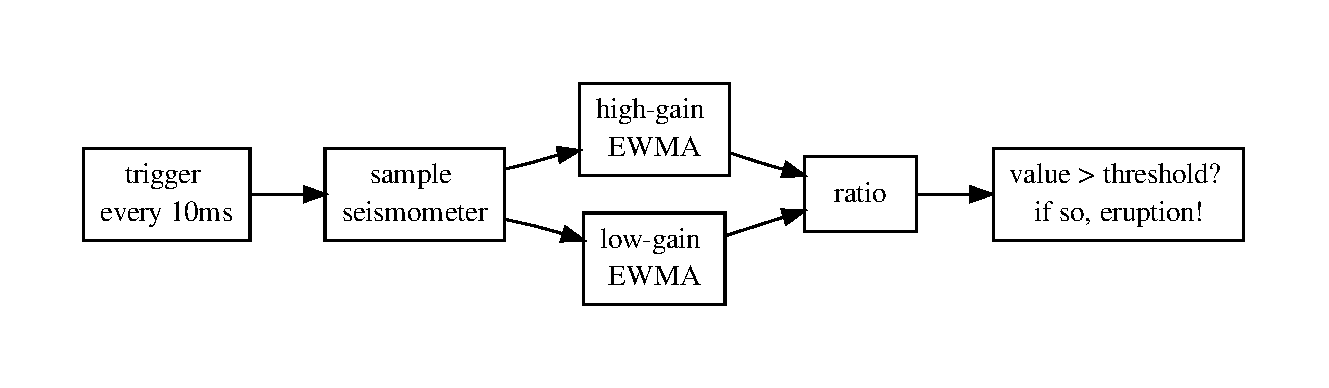
\includegraphics[width=\textwidth]{images/flask-ewma}
  \centering
  \caption{Flask dataflow graph}
  \label{fig:ewma-example}
\end{nonfloatingfigure}

Later we will examine how this is written (or \textit{wired}) in
Flask. We see that this is a single connected graph\footnote{This is
  actually two different \textit{atomic subgraphs} because of the
  special \textit{posting wire} required to use the sensor, but for
  simplicity we won't discuss this now. Refer to \cite{flask06} or our
  \Fref{sec:posting wires} about posting wires.}, but many Flask
programs will consist of several \textit{atomic subgraphs}. We say
that they are atomic in the sense that they have to run to completion
before we can go on to the next action, thus ensuring that any mutable
state they encapsulate is atomically manipulated.  The details for
this notion, as well as details about its implementation, can be found
in \Fref{sec:dataflowevaluationstrategy} and
\Fref{sec:dataflowtranslation}.  An example here is that we might want
two different \textit{atomic subgraphs} to execute depending on
whether a button on our circuit was pushed or released.

\section{From Flask to sensor network-code}
A fundamental aspect of Flask is its compilation and
execution-strategy. A Flask program is a description of the prior
mentioned dataflow-graph written in Haskell, using specialised
Haskell operators (dataflow-operators, stream-combinators,
stream-operators or signal-functions) for connecting and
manipulating the streams. Some of the these stream-operators also
accepts some node-level code which should be inserted into the
dataflow. This node-level code is written in one of several
object-languages (where Haskell is the meta-language) for
manipulating node-level values.

When compiling the Haskell program description of the dataflow graph,
you end up with an executable that generates and outputs code in a
sensor network language called NesC\footnote{NesC is an extension to
  C, with some additional constructs suitable for low-level sensor
  network programming for TinyOS.} \cite{nesc}.

The generated NesC code can then be translated by an ordinary
NesC compiler to machine code running on the nodes in the
sensor network.  Thus, when you write a Flask-program, you use
ordinary Haskell constructs to manipulate which NesC-code should
ultimately be generated.

\begin{nonfloatingfigure}
  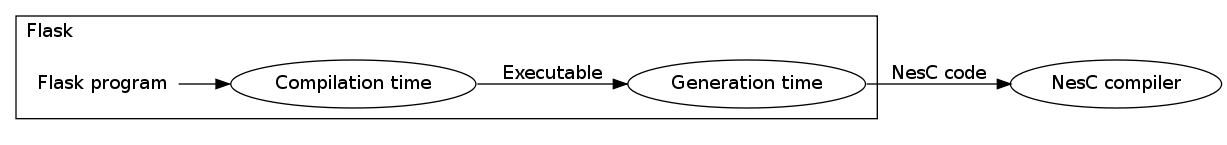
\includegraphics[width=0.9\textwidth]{images/flask-simple}
  \centering
  \caption{High-level illustration of the Flask compilation strategy.}
  \label{fig:flask-simple}
\end{nonfloatingfigure}

Flask provides two object-languages: NesC and Red. Having NesC as an
object-language, allows the user to write all programs that are
expressible in NesC, and NesC is also heavily used as object-language
in the Flask-implementation. The other object-language, Red, is
described in the next section (\ref{sec:red}).

Both languages are integrated into Flask using the GHC quasiquotation
library \cite{quasiquote07}, written by the Flask-author, Geoffrey
Mainland. The quasiquotation facility permits the writing of
object-languages in their original syntax inside the Flask/Haskell
environment, as well as allowing interspersing generation time
variables (which results in compile time constants) into
object-language code.

\Fref{fig:mainloop} illustrates this, showing a simplified
version of the main loop and initialisation code from Fladuino.
\texttt{topdefs} and \texttt{initstms} are generation-time values
(lists of C statements). And \texttt{\$edecls} and \texttt{\$stms} are
\textit{anti-quoters} which at generation-time inserts the values into
the correct position in the C syntax tree.

\begin{figure}
\begin{verbatim}
[$cunit|
$edecls:topdefs

void setup() {
    $stms:initstms
}

void loop() {
    if (event_available()) {
        handle_event(pop_event());
    }
}
|]
\end{verbatim}
\caption{Simplified version of the Fladuino main-loop and
  initialization code.}
\label{fig:mainloop}
\end{figure}

\section{Red --- a restricted node-level language}
\label{sec:red}
Red is an object-language from Flask that allows you to write concise
node-level mapping functions, like predicates or conversion functions
for simple tasks, without having to deal with NesC. It takes its
syntax from Haskell, but is restricted to a small subset of what is
normally expressible in Haskell. The reason for disallowing these
things are the same as for not compiling Haskell directly to the
sensor nodes in the first place: the existing Haskell runtimes are too
large to fit on the limited memory of a sensor node. Therefore we
disallow features that for example requires a garbage collector. Flask
disallows the following Haskell 98-features from Red:
\begin{itemize}
\item Recursive functions
\item Recursive datatypes
\item Curried functions (except for a few simple cases)
\item Higher-order functions
\item Type classes
\item Laziness
\item Modules
\end{itemize}

Furthermore, only a small subset of the Standard Prelude is included
in Flask, and the use of impure functions is prevalent.  In fact, the
semantics of Red feel more like a restricted dialect of Standard ML,
than of Haskell.

Figure \ref{fig:redqq} is an example of a quasiquoted function in Red,
which determines whether a ratio between two values is below a certain
threshold. The threshold could be a generation-time computed value, which is
inserted by the \texttt{flo}-antiquoter (float) at generation-time.
\begin{nonfloatingfigure}
\begin{verbatim}
[$exp|\(hi, lo) -> hi / lo > $flo:threshold|]
\end{verbatim}
  \caption{Example of quasiquoted Red function}
  \label{fig:redqq}
\end{nonfloatingfigure}

\newpage
\section{Streams, node-level values and dataflow-operators}
Expressing dataflow graphs in Haskell is often done using the Arrows
library. But this isn't a strategy applicable to Flask, as the
\textit{Arrow} type class requires that arbitrary Haskell functions
can be lifted to a signal function. This lifting is impossible with
Flask, because the signal-functions of Flask are to be executed on the
sensor nodes and therefore aren't Haskell functions per se, but
instead a representation of the node-level code that should be
generated. Flask still defines some of the same operators as in the
Arrows library, though with different type signatures. Writing
dataflow graphs in Flask therefore still feels quite the same as when
using the Arrows library, but is not able to use the Arrow syntax
(introduced in \cite{PatersonRA:notation}).

In Flask a stream of type $a$ has the type \texttt{S $a$}. The
arguably simplest way to generate such a stream is the Flask-function
\texttt{clock :: Int -> S ()}, which given a time interval in
milliseconds returns a stream of unit signals, that is sent with the
given frequency. For example \texttt{clock 1000} is signalling every
second. This isn't beneficial in itself, but it is useful for activating
other tasks, like reading a sensor at some frequency.  Node-level
code of type $a$ has the type \texttt{N $a$} in Haskell.  For example,
a node-level expression evaluating to an integer is referred to as
\texttt{N Integer}, and a stream of such integers would have the type
\texttt{S Integer}.

We also need to process these signals, and as mentioned before, Flask
provides a set of general stream operators for this task.


\subsection{\texttt{Reify} and \texttt{LiftN}}
Before we go on to explain the stream operators, we need to discuss
two Haskell type classes: \textit{Reify} and \textit{LiftN}.
Instances of the \textit{Reify} type classes are Haskell types that
have node-level equivalents. An instance \texttt{Reify $a$} has to
provide a function \texttt{reify :: $a$ -> Type} that, given a Haskell
value of type $a$ returns a representation of its node-level type.
The actual value is never used, only its type, so a common value to
use is \texttt{undefined :: $a$}. \hfill

\textit{LiftN} is a multi-parameter type class\footnote{This requires
  the GHC language extension MultiParameterTypeClasses.}. An instance
\texttt{LiftN $eta$ Integer} declares that a Haskell value of type
$eta$ can be lifted to code of node-level type \textit{Integer} (by
the function \texttt{liftN :: $a$ -> N $a$}).  This lifting is notably
used to lift quasiquoted Red function definitions to
node-level code that can be called by the final node-level program.\\

\noindent
Let us consider an actual Flask stream operator, namely
\texttt{sfilter}. An informal description of its purpose is that it
accepts a stream of values as its input, and passes those values, that
satisfy some predicate, onwards as output.  Its type signature is:

\begin{verbatim}
sfilter :: forall a eta . (Reify a, LiftN eta (a -> Bool))
              => eta -> S a -> S a
\end{verbatim}

Thus the stream operator \texttt{sfilter} takes as its first argument
any value that can be lifted to a node-level function of type
\texttt{a -> Bool} (a predicate function), and returns a signal
function (\texttt{S a -> S a}) that for each input value uses the
predicate to decide whether it should be passed on to its output
stream or not.


\subsection{Stream-operators}
\label{sec:streamoperators}
In this section we will describe the stream-operators and signal
functions that Flask provides. This also serves as a small
documentation of Fladuino, as the same stream-operators are available
in Fladuino.

\begin{description}
\item
\begin{verbatim}
sconst :: forall a b eta. (Reify b, LiftN eta a)
       => eta -> S b -> S a
\end{verbatim}
  \texttt{sconst} maps all values on the input-stream to a constant (node-level) output value.

\item
\begin{verbatim}
(>>>) :: forall a. Reify a => S a -> (S a -> S a)
\end{verbatim}
  Connects a stream with a stream operator.  For example {\ttfamily clock 10 \verb|>>>|
    sconst (liftN [\$exp|42|])} is an infinite stream of 42 values, that is passed on
  every 10th millisecond. This is simply implemented as a Haskell function
  application.


\item 
\label{item:szip}
\begin{verbatim}
szip, (&&&) :: forall a b . (Reify a, Reify b)
      => S a -> S b -> S (a, b)
\end{verbatim}
  This operator has two input-streams. It waits for a value on both
  inputs, constructs a pair of them, and sends this pair to its
  output-stream.  Should several signals arrive on one of the inputs
  before one arrives on the other, the most recently arrived value
  will be used.

\item 
\begin{verbatim}
sunzip :: (Reify a, Reify b) => S (a, b) -> (S a, S b)
\end{verbatim}
  The inverse of \texttt{\&\&\&} and \texttt{szip}, which splits a
  stream of pairs into two individual output-streams.

\item 
\begin{verbatim}
smap :: forall eta a b . (Reify a, Reify b, LiftN eta (a -> b))
  => eta -> S a -> S b
\end{verbatim}
  Maps a node-level function over all stream-values, creating a stream
  of the resulting output-values.

\item
\begin{verbatim}
sintegrate :: forall a b c eta . (Reify a, Reify b, Reify c,
                              LiftN eta ((a, c) -> (b, c)))
       =>  N c -> eta -> S a -> S b
\end{verbatim}
  \texttt{sintegrate} is the primary state-retaining stream operator.
  It maps a tuple $(x, s)$, where $x$ is a newly arrived
  value and $s$ is the state, to the tuple $(y, s')$, where $y$ is the
  output value and $s'$ is the new state.  The $N c$ argument in the
  type signature is the initial state.

\item
\begin{verbatim}
clock :: Int -> S ()
\end{verbatim}
  Creates a stream of unit-values
  that is fired with the given interval (specified in milliseconds).

\item
\begin{verbatim}
sfilter :: forall a eta . (Reify a, LiftN eta (a -> Bool))
     => eta -> S a -> S a
\end{verbatim}
  Only propagates values through to the
  output-stream that satisfies a given node-level predicate.
  
\item
\begin{verbatim}
smerge :: forall a . Reify a
    => S a -> S a -> S a
\end{verbatim}
Takes two input streams of the same type. When it received a value on
either of the inputs it will propagate this value to its output, thus
merging the streams into a single stream.

\end{description}
\newpage
\section{From dataflow graph to Flask-code}
The dataflow graph from \Fref{fig:ewma-example} can now be written
in Flask like below (the code is an almost verbatim copy from
\cite{flask08}). The result is a stream that only produces values when
an earthquake is detected.
\begin{verbatim}
detect :: Double -> Double -> Double -> S (Double, Double)
detect low high threshold = 
     clock 10
   >>>
     adc "Seismometer"
   >>>
     ewma high &&& ewma low
   >>>
     sfilter [$exp|\(hi, lo) -> hi / lo > $flo:threshold|]
\end{verbatim}

\noindent
The function \verb#adc :: String -> S () -> Double ()# is a Flask
built-in operator for reading sensor-values, the String-argument
specifies which NesC interface to use for querying the sensor.

The function \texttt{ewma} retains an exponentially weighted moving
average with the given gain, which is updated for each input
value. Its implementation in \cite{flask08} follows:

\begin{verbatim}
ewma :: Double -> S Double -> S Double
ewma gain = sintegrate zero
               [$exp| \(x, xold) ->
                        let x = $flo:gain * x +
                                (1.0 - $flo:gain) * xold
                        in (x, x) |]
    where
      zero :: N Double
      zero = liftN [$exp| 0.0 |]
\end{verbatim}



\chapter{Design of the Fladuino system}
\label{chap:design}

In this chapter we shall outline the overall design of Fladuino, as
well as present some of the technical decisions that have a notable
impact on how Fladuino is used.  Technical details that have less of
an impact on the final usage of the system are described in
\Fref{chap:implementation}.

Fladuino is a modification of Flask that can be used to program
Arduino devices in a functional reactive manner. In this chapter we
will analyse which requirements we need to set and which design
choices should be made.

A summary of the most important requirements for our system follows:

\begin{itemize}
\item It must be possible to define interfaces to external devices
  connected to an Arduino board, without having to modify Fladuino
  itself.  Interaction with these devices must take place through the
  same statically typed stream operator (and event) interface as any
  built-in part of Fladuino.
\item It must be possible to define simple variations on Arduino
  boards in terms of I/O-pin availability and custom capabilities,
  without having to modify Fladuino itself.  Implementing support for
  platforms that differ significantly from our built-ins (for example,
  using a different microcontroller) however, will not be possible without
  modifying the Fladuino libraries.
\item Fladuino must statically analyse and validate the program for
  certain classes of type and logic errors.
\item Fladuino must be able to generate a valid C-program suitable for
  running on the Arduino platform from a description of a dataflow graph. This
  graph must be expressed in the form of a Haskell program.
  \footnote{This requirement stems from the selection of
    Arduino (see \Fref{sec:hardware platform}) as platform.}
\end{itemize}

And we set the scope of our project as follows:
\begin{itemize}
\item The design of Fladuino must mirror similar core design choices
  in Flask.
\item We do not have to attempt to handle all error conditions.  We
  accept that hardware constraints pose certain hard restrictions
  (such as memory limits, integer counter overflow and CPU time
  starvation), and declare that writing a program with Fladuino that
  exceeds these constraints will result in information loss or
  undefined behaviour.  We shall, however, endeavour to design
  Fladuino so as to reduce the likelihood of these errors.
\item As we see this as a research project rather that an engineering
  project, we won't devote time to writing documentation for Fladuino.
\item A notable last narrowing of our scope is that we won't provide
  primitives for programming real time systems.
\end{itemize}

\section{Design foundations}

This section will summarise the basic structure of Fladuino, its
terms, and the constraints under which the design was formed.

\subsection{Terminology and basic \textit{modus operandi}}

As in Flask, Fladuino is implemented as a set of Haskell modules that
provide facilities for expressing the structure and behaviour of a
\textit{dataflow graph}, connecting \textit{dataflow operators}
through value-carrying directed graph edges (\textit{wires}).  The
programmer writes a Haskell program, called the \textit{generator
  program}, or just the \textit{program}.  We shall refer to the
compilation of the program as \textit{compile-time}, and execution of
the program as \textit{generation-time}.  At generation-time, the
output will be a program source file suitable for further compilation
with the Arduino tools, but these are not part of the Fladuino system.

\subsubsection{Note on error detection}

Generation-time may also terminate erroneously if the program contains
static errors: in this case, an error message with a description of
the problem will be printed.  Only errors that are violations of the
Haskell type system can be caught at compile-time, and while we have
attempted to structure the facilities provided by Fladuino such that
invalid programs will contain type errors, this cannot be done for all
error classes.  When the generator program is run, it constructs a
typed dataflow graph.  However, the types and connections in the graph
cannot be known in advance (they may be determined
pro\-gram\-mati\-cally, perhaps even by user input), hence we may
signal type errors at generation time if the wiring of stream
operators violate type-safety.  We do, of course, supply Haskell
operators operating on stream representations with assigned static
types, that guarantee the type-validity of the resulting graph, but
certain sophisticated applications of Fladuino may desire more
flexibility than permitted by these.  This is notably the case when
the structure of the graph is a function of a value not known until
generation-time (and thus can't possibly be checked by the Haskell
compiler at compile-time).

It is intended that all static errors are caught at compile- or
generation-time; in particular that Fladuino will never generate
malformed C.  This guarantee does not extend to C code manually
included or integrated by the user, of course.

\subsection{Hardware constraints}

While we do not use Arduino to refer to any specific hardware
configuration, implementations of our target platform still share some
fundamental characteristics that have influenced many design choices
and tradeoffs in Fladuino.  In particular, the low amount of available
main memory, and the comparatively large amount of available flash
memory for program code, suggests that we optimise for low memory
usage over low code size.  Indeed, as we shall see in
\Fref{sec:dataflowtranslation}, we have opted to directly express much of
the control flow in the code itself, where a typical program, with
plenty of available memory, might instead opt a more data-driven
approach.  This choice was also made in Flask itself, and as
\cite{flask08} observes, such static dataflow is not a problem for a
large class of applications.  Additionally, we recover much of the
lost flexibility through programmatic wiring of the dataflow graph at
generation-time.

\section{Structural overview}

Fladuino consists of several interconnected parts combined to form a
domain-specific language embedded in Haskell.\footnote{We do however
  make heavy use of Glasgow Haskell language extensions, such as
  multi-parameter typeclasses and existential types, so Fladuino will
  not run in a standard implementation of Haskell 98.}  As in Flask,
this takes the form of providing facilities to express the structure
of a \textit{dataflow graph}, connecting \textit{dataflow operators}
through directed graph edges (\textit{wires}).  Conceptually, these
parts can be divided into the following:

\begin{itemize}
\item Haskell operators and functions used to describe the dataflow
  graph have been defined.  It is not intended that these are
  exclusively used to construct the program, but rather that they are
  part of a larger Haskell program.  Since a Fladuino program is
  highly static at run-time, the generating program should be written
  to support easy configuration and modification.
\item A compiler is supplied for the Haskell-like programming language
  Red (see section \ref{sec:red}), which is used to tailor the
  behaviour of stream operators.
\item A \textit{stream generator} that takes a description of a
  dataflow graph and generates object code (in the case of Fladuino,
  C).
\item The \textit{Fladuino runtime system}, consisting of code written
  in C implementing the runtime facilities used by the generated code.
  The most notable part of the runtime system is the event loop and
  its supporting machinery, which is the subject of
  \Fref{sec:dataflowevaluationstrategy}.
\item A module that encapsulates the hardware facilities offered by
  the target platform and provides the ability to check whether the
  requirements made by the users program can be fulfilled.  Arduino is
  a highly variable hardware platform, no more than a simple
  microcontroller connected to a basic extensible circuit board, and
  no assumptions can be made about which electrical components the
  user might need to control.  Therefore we provide a comprehensive
  facility for expressing device interaction in a high-level fashion,
  and automatically check whether any of these interactions are
  incompatible, or violate basic hardware restrictions.  For example,
  we might check that the program does not try to interact with a
  pushbutton connected to a hardware pin that does not support
  interrupts, or that the program does not express both a
  potentiometer and diode connected to the same pin.\footnote{Of
    course, it must be mentioned that we cannot possibly check that
    the hardware has actually been set up in the way described by the
    program --- we can only check for internal consistency and
    violations of basic hardware restrictions, not whether the
    programs model of the device actually corresponds with reality.}

  Furthermore, since there are several different boards under the
  Arduino name, all with slightly different capabilities, we permit
  selection of the exact Arduino variant targeted by the program.

  Finally, since Arduino is a fundamentally extensible platform, we provide
  facilities for implementing drivers (see \Fref{sec:user-extens-abstr}) for
  entirely new devices, in a way that use of these is also automatically
  sanity-checked.
\end{itemize}

Except for the last module, this structure has been adopted from
Flask.  Furthermore, Flask defines additional facilities (such as
\textit{Flows} for communicating between sensor nodes) that build
heavily upon the TinyOS-platform for sensor networks, a platform that
is not available to us.  We have thus not adapted all of these
facilities in our work.  Posting wires, however, (see
\Fref{sec:posting wires}) have their own novel implementation in
Fladuino.

\section{Dataflow evaluation strategy}
\label{sec:dataflowevaluationstrategy}
As in Flask, the dataflow graph is divided into \textit{atomic
  subgraphs} consisting of a set of nodes connected by normal wires.
Evaluating such a subgraph consists of supplying a value on the input
wire, retrieving any values that may show up on output wires, then
setting up to evaluate any of the successor atomic subgraphs with
these values (see \Fref{sec:dataflowtranslation} for the
implementation details).  The notion of an atomic subgraph serves the
purpose of dividing the dataflow graph into parts that can be
evaluated atomically without blocking.  Translating a dataflow graph
into object code is referred to as \textit{stream generation}.
Translating an atomic subgraph is relatively straightforward, and is the
subject of \Fref{sec:dataflowtranslation}, while it is far more
interesting to contemplate the question of what to do with the
asynchronous events that are the heart of reactive programming.
Indeed, we have to analyse the constraints of our target platform(s)
in order to reach an adequate solution.  Since events are
fundamentally connected to the concept of a hardware interrupt (though
we do not reject the ability to manually signal synthetic events --
software interrupts, if you will), we cannot at any time predict, or
control, their arrival.

The simplest strategy would be to, upon arrival of an event via an
asynchronous hardware-level interrupt, immediately evaluate all atomic
subgraphs that have nodes listening to the event.  However, this
approach is unacceptable for several reasons:

\begin{itemize}
\item If we are already in the progress of computing an atomic
  subgraph $s_1$, we will have to store information about the
  computation while we evaluate all graphs $s_n$ listening to the
  newly arrived event.  The size of this information can be
  significant, especially if we receive yet another event while
  evaluating one of $s_n$.  There is no upper bound on the number of
  events we can be forced to handle within each other, and the storage
  spent on saving the state of each computation can be significant on
  such memory-constrained devices as the Arduino platform.
\item Doing large computations (in space or time) within interrupt
  handlers is generally a bad idea.  Not only are additional
  interrupts disabled while running the handler (and making them
  re-entrant is nontrivial), but the already running code may already
  tie up an arbitrary amount of the memory resources.  As a result,
  interrupt handlers should ideally terminate swiftly and use few
  resources, which cannot be guaranteed for evaluation of arbitrary
  atomic subgraphs.
\item Most importantly, the subgraph computation already in progress
  may be in a critical section, and we cannot guarantee that the
  subgraphs to be evaluated in response to the event will not overlap
  with this critical section.  Thus, we can end up with interleaved
  access to explicit state (memory contents) as well as implicit state
  (output).  This violates one of the basic tenets of atomic
  subgraphs, namely atomicity of computation.
\end{itemize}

As a result of the previously mentioned considerations, our basic
program evaluation is as follows.  We shall maintain an ordered
\textit{event queue}, each element containing information about an
atomic subgraph (actually, an entry node to the subgraph) that should
be called, as well as the input value that caused the input wire to
fire.  The generated program consists of a loop that continuously
checks for the presence of an element in the queue, and if so, removes
it and computes the subgraph indicated by it.  Hardware interrupts are
handled by checking all events that may be signalled by the given
interrupt (the details of this check are defined individually by each
type of event), and if the check is positive, an element is added to
the event queue requesting the evaluation of all listeners of that
event.  It is important that the event-check, as well as the
computation of the value of the event, is done in the interrupt
handler itself, as the value may depend on the hardware state (such as
the voltage on an input pin) as of that moment and it cannot be
guaranteed that this state has not changed by the time the main loop
retrieves the element from the event queue.  This means that we cannot
provide any strict guarantees about the resource usage of interrupt
handlers, but this is a hardware issue that is not solvable in
software.  Optimisations can be performed, of course, but ultimately
there are constraints on how much any computer can do.

\begin{figure}
\begin{verbatim}
repeat forever
  if (event_available())
    handle_event(pop_event())
  endif
endrepeat
\end{verbatim}
\caption{Pseudocode for the event loop}
\label{fig:eventloopcode}
\end{figure}

\subsection{Idle waiters}
\label{sec:idle waiters}
For many embedded applications, a typical workflow would be to
continuously poll an input source (such as a sensor), then adjusting
some output device based on the reading.  For example, a
line-following robot (as the previously mentioned Pololu 3pi) may take
readings from its light sensors, then adjust its servo-motors to
ensure that it is following the line straightly.  This can be done by
simply attaching a node to a clock that fires every millisecond, but
this approach has a notable disadvantage if many other events are
being received at the same time.  The event queue may become filled
with a large amount of clock events, thus drowning out (and losing)
potentially more interesting events.  In most cases, it is not a
problem that the continuous polling of the input source is in
irregular intervals, but the silent loss of events such as button
presses is normally undesirable.

Thus, we provide the notion of \textit{idle waiters}, a list of atomic
subgraphs that are evaluated in a round-robin fashion whenever the
event queue is empty.  They are a useful facility for specifying
computations that should be done whenever the program is not busy with
something else.

\subsection{Posting wires}
\label{sec:posting wires}
In the dataflow graph, atomic subgraphs can be connected by
\textit{posting wires}.  These serve to temporarily suspend execution
while the system waits for external response, thus serving in place of
blocking operations (which are not permitted in atomic subgraphs).
Conceptually, when a posting wire is encountered during evaluation of
the graph, it will send a request to an external hardware unit, wait
for a response, and then fire the destination node with the value of
the response as the input value.  Posting wires are therefore a
natural fit for solving the problem of sensor-requests that can
involve waiting an indeterminate time for the response.  For clarity,
in the following we shall refer to the external device as the
\textit{sensor}, the node preceding the posting wire as the
\textit{input node} and the node following the posting wire as the
\textit{output node}.  The phrase \textit{send a request to the
  sensor} denotes the act of requesting data from the sensor under the
assumption that a reply will be received.  Note that ``output node''
is a lossless abstraction, as several nodes may be on the receiving
end of the posting wire.  A fundamental simplifying assumption we make
in the following section is that the structure of the sensor request
is a function only of the identity of the posting wire, and is notably
not based on the value that arrived at the input node.  This rule,
which is also present in Flask, grants us much more leeway in the
implementation of posting wires.

It is not intuitively obvious what to do when a posting wire is
reached a second time, before a response has come back from the
previously sent request.  Several options present themselves:

\begin{description}
\item[Accumulate-Repeat:] If we are already waiting for a response
  from the sensor for the posting wire when a value arrives at the
  input node, we will not send another request.  Instead, we will
  increase an internal counter, and upon receiving the sensor
  response, fire the output node a number of times equivalent to the
  number of times a value arrived at the input node.  See
  \Fref{fig:accum-repeat} for a visualisation.
\item[Queue:] When a value arrives, queue a request to the sensor.  We
  cannot assume that all sensor hardware supports a request queue (in
  fact, we can be fairly certain that most will not), so we have to
  maintain this queue in the Fladuino runtime system.  Whenever a
  response comes back from the sensor, we fire the output node and
  check whether there are any requests left in the queue.  If so, we
  send it.  As the format of a request is a function of only the
  posting wire itself, not the incoming value, such a queue could be
  implemented as a mere integral counter, thus ignoring the problem of
  dynamically allocating memory (and potential problems resulting from
  such, as described in section \ref{sec:event_queue}).  See
  \Fref{fig:queue} for a visualisation.
\item[Ignore:] We can also opt not to queue or accumulate anything,
  ignore any input values sent while there is already an outstanding
  request, and fire the output node a single time upon receiving a
  reply from the sensor.  This strategy also implies that whatever
  value was carried by the signal that arrived at the input node to
  trigger the posting wire will be lost, unless the user takes care to
  explicitly route it around the wire (the \texttt{szip} stream
  operator described in \Fref{sec:streamoperators} is highly useful
  for this).  While appearing to be a lossy hack at first glance, we
  argue that it is in fact the most elegant solution, that its
  deficiencies are not important in the typical case, and that they
  can (to a degree) be worked around, if necessary.
\end{description}

\begin{figure}
  \includegraphics[width=\textwidth]{images/accumulate-repeat-1}
  \includegraphics[width=\textwidth]{images/accumulate-repeat-2}
  \includegraphics[width=\textwidth]{images/accumulate-repeat-3}
  \caption{Visualisation of Accumulate-Repeat}
  \centering
  \label{fig:accum-repeat}
\end{figure}

\begin{figure}
  \includegraphics[width=\textwidth]{images/queue-1}
  \includegraphics[width=\textwidth]{images/queue-2}
  \includegraphics[width=\textwidth]{images/queue-3}
  \caption{Visualisation of Queue}
  \centering
  \label{fig:queue}
\end{figure}

Both the \textit{Accumulate-Repeat} and \textit{Queue}-strategies
suffer from \textit{clogging-propagation}, where the multitude of
inputs, greater than the sensor is capable of handling, will also
result in a large amount of activity on the output side of the posting
wire.  Especially Accumulate-Repeat suffers badly, as the receiving of
a sensor-reply will result in a potentially large amount of work, a
situation that can result in information loss if the event queue fills
up.  And as each firing of the output node will be with the same
value, it is in practice often unlikely that the repeated evaluations
are appreciably different from just a single evaluation.

The Queue strategy is more appealing, having the attractive property
that every input eventually results in a sensor request and a value
sent to the output node (barring hardware failure or --- unlikely ---
integer counter overflow).  The chief disadvantage is that there is no
way to stop the execution of the queue, should it outlast the
necessity for sensor requests.  A brief flurry of input values might
translate into requests being sent to the sensor long after it is
desirable.  Recall that a sensor request may not necessarily translate
to a harmless, passive reading, but can be everything between reading
a simple light sensor to transmitting a sonar pulse and detecting the
environmental echo.  The Ignore strategy only causes consecutive
requests to be sent to the sensor if the input node keeps receiving
input.  Thus, a posting wire can be considered an abstraction that is
activated as long as it keeps receiving input values, and outputs a
continuous stream of sensor readings as long as it is activated.

\subsubsection{Simulating Accumulate-Repeat and Queue with Ignore}

Should the behaviour exhibited by the Accumulate-Repeat and
Queue-strategies be required for some application, we will
show that it is possible to approximate their behaviour via the
Ignore strategy.  We shall not delve into the gory technical details
(such as the error handling necessary to avoid fragility), but
merely show the structure of the solution.

For Accumulate-Repeat, we can connect both input and output nodes to
an \textit{accumulator node} that distinguishes between its two
inputs.  When receiving a value from the input node, an internal
counter will be increased by one.  When receiving a value (the sensor
reading) from the output node, the value will be packaged up with the
counter into a tuple and sent to successors of the accumulator node,
after which the counter will then be reset to zero.  Said successors
will be the nodes that would normally follow the output node.  This
does not in itself implement the ``repeat''-portion of
Accumulate-Repeat, but we have removed the loss of information, and
can thus trivially take whatever action repeated firings of the output
node would have resulted in.

\begin{figure}
  \includegraphics[width=0.9\textwidth]{images/accum-repeat-with-ignore}
  \caption{Simulating Accumulate-Repeat}
  \centering
  \label{accum-repeat-with-ignore}
\end{figure}

Simulating the Queue behaviour is significantly more complicated and
requires a somewhat clumsy use of events (see
\Fref{sec:events_design}).  Values received at the input-node are sent
on to a \textit{counter node}, where we check whether we are still
waiting for the sensor to reply to a previously sent request.  If so,
we increment an internal counter and send nothing further.  When the
reply is received, by being sent to the output node, we will send a
value to the counter node, telling it to send another request to the
sensor if the counter is nonzero.  The problem in this scheme is the
wire from the output node to the accumulator node --- this graph edge
would form a cycle, something that is expressly forbidden.  On
\Fref{fig:queue-with-ignore}, we solve this issue by an \textit{event node}
that listens to a discrete event broadcast by the output node (the
Fladuino event system is described in detail in
\Fref{sec:events_design}).  Using the event system in such a way is
technically feasible, but violates the spirit of the design.  The
connection from output to event node can be considered to be a
particularly weak kind of posting wire --- informally, they are to
real posting wires, as software interrupts are to hardware interrupts.

\begin{figure}
  \includegraphics[width=0.9\textwidth]{images/queue-with-ignore}
  \caption{Simulating Queue}
  \centering
  \label{fig:queue-with-ignore}
\end{figure}

\section{Representing peripherals} 

Arduino is a flexible system for general embedded development, with no
specific application in mind.  The Arduino platform can therefore be
connected to a diverse amount of peripheral devices, all with their
own specific functionality and programming interface.  It is thus
natural to support this diversity as a core concept of Fladuino; not
(solely) as a library of drivers for various devices, but rather as a
framework and set of tools provided to the programmer so that Fladuino
can be extended to transparently support the devices he has need of.
For demonstration, we have written a minimal framework for programming
the Pololu 3pi robot and \textit{some} of the peripherals connected to
it (electromotors, reflectance sensors, etc.). This framework is
discussed in \Fref[plain]{chap:example code} and evaluated in
\Fref[plain]{chap:evaluation}

Furthermore, Arduino is a broad term encompassing a range of
more-or-less compatible platforms, though each of them differ slightly
in their exact capacity.  Apart from variations in such things as
memory size, they differ in amount and capability of their I/O pins.
This latter diversity is what we are most concerned about in Fladuino,
as we would like to statically check (at generation-time) the hardware
assumptions expressed in the program.  Thus, we also provide a
facility for describing the exact capabilities of a specific
Arduino-based platform, and provide default descriptions of common
Arduino-compatible such as the Arduino Duemilanove, Arduino Mega,
Arduino BT, and Pololu 3pi.

% Defining the driver for each external component consist of a general
% device specification in the form of a Haskell type definition, a set
% of functions operating on the device type, and possibly a set of event
% specifications, provided the device supports the notion of events.

% \fixme{find a good example to add here}

\subsection{Platforms}
\label{sec:platforms}

Arduino is a heterogeneous ecology.  Apart from the various models
that differ in availability of I/O pins, processor speed and available
program memory, there are also highly specialised variants such as the
Arduino BT with a built-in bluetooth module, and the Pololu 3pi, a
mostly Arduino-compatible robot designed for line-following.  The
primary difference between these variants is their availability of
I/O-pins, a difference that we must be reflected in Fladuino if we are
to sanity-check device use.  Additionally, some platforms (such as the
previously mentioned Arduino BT) have additional intrinsic qualities,
like the built-in Bluetooth module, that must be expressed somehow,
such that attempts to use said Bluetooth device will be erroneous
unless we are compiling for an Arduino BT.

A platform is defined by a list of \textit{logical pins} (described in the next
Section), and free-form \textit{capabilities}, the latter being a set of strings
describing the identity or unusual qualities of the platform.  For instance, the
platform definition for the Pololu 3pi robot contains a ``3pi''-capability that
exists merely to express the fact that the platform supports the quirks of the
3pi robot that cannot be expressed through a list of pins.  Any device intended
to make use of these quirks would explicitly require the presence of this
capability.

\subsubsection{The Fladuino pin model}
\label{sec:pins}
There is no concrete distinction between analog and digital pins in
the Atmel microcontroller that lies at the heart of all Arduino
platforms --- they are just subsets of the single set of numbered pins
that differ in their capabilities.  Arduino, however, drives a hard
distinction between analog input and general-purpose digital pins, in
particular enumerating them in different sequences (there is a digital
pin 0 distinct from analog pin 0).  This notion is fully integrated
and supported in Fladuino; in fact there is no way to directly address
pins by the name they are known by to the Atmel microcontroller.  We
identify three layers of pin abstraction, each building on the one
below it:

\begin{description}
\item[Arduino pins] are what a normal user of Arduino will be familiar
  with.  They are identified by a \textit{pin type} (digital or
  analog-input) and a number.  Analog-input pin 0 and digital pin 0
  are not the same pin.  This is the layer of abstraction that devices
  work at.
\item[Logical pins] are a simplification of Arduino pins, where the
  Arduino pin abstraction is mapped to a single enumerated sequence.
  This mapping is defined specifically for each platform; for example,
  Arduino digital pin 0 will equal logical pin 0 on both the
  Duemilanove and Mega platforms, but analog pin 0 equals logical pin
  14 and 54, respectively.  A typical user of Fladuino will never have
  to go below this level of abstraction, and will only have to
  interact with it if he is defining a new platform.
\item[Hardware pins] are the physical pins connected to the
  microcontroller.  They are only interacted with in the
  implementation of the Arduino and Fladuino supporting libraries.
  The Arduino libraries themselves define the mapping from logical to
  hardware pins, and adding a new mapping is a significant task.
\end{description}

This choice of abstraction is not as obvious as it may appear: some
measure of expressive power is lost by restricting ourselves to the
interface provided by Arduino, rather than permitting complete
exploitation of the capabilities of the microprocessor.  Yet for the
following reasons, we believe we made the right choice:

\begin{itemize}
\item The software abstraction provided by Arduino exposes a uniform
  interface to a range of different hardware implementations.  These
  implementations share a similar software interface to their shared
  functionality, thus making porting between them easy.  In contrast,
  not even pin numbers are necessarily identical between the
  microcontrollers found across the range of supported platforms.  We
  could solve this by defining our own mapping between abstract pins
  and hardware pins (based on the chosen platform), but we see no
  advantage to this approach over adopting the mapping already defined
  by Arduino.
\item A shared pin abstraction makes it easier for Fladuino-generated
  programs to use existing Arduino libraries.
\item The pin identifier sequences defined by the Atmel
  microcontrollers are not particularly intuitive when mapped to the
  physical layout of the Arduino boards.  They are fragmented and with
  large jumps.
\end{itemize}

Abstractions aside, each pin is not only defined by its number, but
also by a set of \textit{capabilities}, much like the ones that cover
the entire platform.  For example, a given pin may support such things
as logical change \texttt{interrupts} (triggering an asynchronous signal
when the input value on the pin changes) or \texttt{pulse width
  modulation} (analog output).  Many hardware devices only work when
attached to pins with special capabilities --- for example, a
push-button must be attached to a pin supporting interrupts --- and
the capability notion allows us to statically sanity-check any used
devices for such requirements at generation-time.

\subsection{Devices}
\label{sec:devices}
We use the term \textit{device} for any form of peripheral that can be
connected to an Arduino board; for example buttons, electromotors and
potentiometers.  A device-driver consists of a list of
\textit{usages}, each describing a discrete reservation of some
hardware resource, a function for initializing the device and possibly
a set of functions for interacting with the device.  A device can be
parametric --- in fact, most are --- in for example the I/O pins that
it is attached to.  As a concrete example, the device describing a
plain digital output pin is parametric in the form of the single
integer parameter denoting the number of the digital pin it
represents.

The notion of a usage deserves further elaboration: apart from being a
facility for statically finding resource usage conflicts between
devices, they serve as a way to configure the starting state of the
Arduino board.  We define three different kinds of usages, two of which
reserve exclusive access to the hardware resource that they refer to:

\begin{description}
\item[Digital pin usage] is an expression of exclusive access to one
  of the digital pins on the Arduino board.  If any other device has a
  usage involving the same pin, this will be reported as an error at
  generation-time.  A digital pin usage also specifies a list of
  capabilities that must be provided by the indicated pin.
  Additionally, a digital pin usage can have one of three types:
  \begin{description}
  \item[Digital output,] in which case the usage will also have to
    specify a starting value (\texttt{HIGH} or \texttt{LOW}) on the
    pin.
  \item[Digital input]
  \item[Analog output,] in which case a starting value must be
    specified in the range $[0,255]$.  Note that this ``analog'' value
    is, of course, implemented via PWM (see \Fref{sec:pwm}), and the
    capability ``PWM'' should thus be required of the pin.
  \end{description}
\item[Analog input pin usage] denotes exclusive access to a specified
  analog input pin.  The usage also specifies a list of capabilities
  that must be provided by the indicated pin.
\item[Capability requirement usage] is a dependency on the presence of
  a given \textit{platform capability} (see \Fref{sec:platforms}).  In
  contrast to the pin usages, this dependency is not exclusive.
\end{description}

Some measure of power is lost by restricting devices to exclusive
access to pins.  However, the fragility of having devices share these
I/O pathways require detailed knowledge of exact device behaviour
anyway, in order to ensure that they will not be incompatible.  Given
this knowledge, the user can merely connect several physical devices
to the same IO pin (for example, multiple diodes to the same digital
output pin) and use a single logical device in the Fladuino program to
interact with them.  Indeed, this solution is mostly satisfactory, as
long as the devices are (almost) identical in their interface.

See \Fref{sec:pushbuttondef} for an example of how to define a device
via these abstractions.

\subsection{Events}
\label{sec:events_design}
A central aspect of any embedded system is responding to external,
asynchronous events.  The hardware feature enabling this functionality
--- asynchronous interrupts --- is primitive and hard to use, leading
us to define a high-level interface, closely interconnected with the
device abstraction, with which we can describe reactions to stimuli in
terms that are closer to the problem domain of the application.  In
the following, we distinguish between \textit{triggering an
  interrupt}, which is the hardware executing the interrupt handler,
and \textit{triggering an event}, which is Fladuino arranging for the
execution of any event listener operators with the event as the input
value.

All events have a static type and value, which is used to distinguish
between them at generation-time, and an event may carry a data
\textit{payload} at runtime.  A critical piece of static information,
that can be found in most (if not all) events, is the device that the
event is associated with.  In our exposed programming interface, all
events stem from external sources of input, and a given event is such
intrinsically linked to some specific device, though it is possible to
define events that are not connected to Arduino's notion of a logical
device --- for example, by hardcoding the I/O pins directly into the
implementation of the event.  ``Synthetic'' events, events that are
explicitly triggered by stream operators, are not conceptually
problematic (apart for the need to distinguish same-type events by
something else than an associated device), but for reasons of time,
Fladuino does not expose a programming interface for triggering them.
We believe that manually triggered events open some interesting new
possibilities (one being Turing--completeness for
dataflow programs) but we could not afford them the attention they
deserve without straying too far in scope from the topic of our
project.

In this section, we shall assume that all events are connected to
Fladuino's notion of a device.  Not all events have payloads (or
rather, some events have payloads of the information-less type
\textit{unit}): an event indicating the press of a pushbutton has no
payload, and contains no information apart from the static event value
itself (which indicates the exact button that was pressed), while an
event indicating that a piece of sensor hardware has finished
performing a reading may contain the reading data as payload.

As an example, assume that $p_1$ is a pushbutton device connected to
digital pin 1, $d_2$ a diode connected to digital pin 2, and $\sigma(e,d)$ a
dataflow graph node that fires whenever the given device $d$ triggers
event $e$.  We can then construct a dataflow graph such as
$\sigma(pushdown,p_1) \rightarrow toggle(d_2)$, connecting the input
of pressing a button to the action of toggling the state of a diode.

In the definition of an event, a list of Arduino pins (see \Fref{sec:pins})
indicates which logical-change interrupts might trigger the event.
Additionally, two object-language functions are defined: a
\textit{predicate}, for checking whether a given pin-change interrupt
should actually cause the event to trigger, and a
\textit{value function}, that calculates the payload (if any) of the
event.  This yields total control to the event implementor, at the
cost of having to check all events possibly triggerable by an
interrupt, whenever the interrupt is triggered.  This can potentially
be problematic: as mentioned above, it is highly undesirable to spend
too much time in an interrupt handler, but we cannot defer execution
of either predicate or value function, as the result of those may
depend on highly volatile dynamic state of the Arduino.  Indeed;
merely the minute delay between the triggering of the interrupt, and
the execution of a some predicate or value function, may change this
state.  On the upside, the time spent in the interrupt handlers will
have a static upper bound defined by the number of events used in the
program, thus making problems of this sort likely to appear during
initial testing, and not lay dormant until after deployment.  Of
course, this bound is dependent on the implementation of the
user-defined predicate and value functions --- if these have
unpredictable runtime behaviour (or worse: block), we cannot guarantee
anything.  See \Fref{sec:pushbuttondef} for example code.

Events initiate dataflow at nodes marked as \textit{listeners} for the
specific event.  Design-wise there is nothing that prevents these
listeners from being successors of other nodes in some atomic
subgraph, but we have not been able to identify a general use for such a
structure during our work (though see \Fref{sec:postingwireimpl} for a
notable exception).  As a result, we generally consider an
event-listening node to have no way of firing except for the
triggering of one of the events that the node is listening for.  A
single node can listen to multiple different events (though again, we
have not been able to identify a practical need), as long as the
payloads are of the same type.

\section{The runtime system}
\label{sec:runtime-system}

Fladuino is not only a code-generator, it also contains a runtime
system that implements much of the complex behaviour that the
generated code expresses.  This runtime system not only has to respect
the constraints imposed by the Arduino hardware, but also run
sufficiently fast while implementing the facilities necessary for the
Fladuino-generated code.  We need several facilities apart from what
is provided by the Arduino libraries themselves:

\begin{itemize}
\item We must have a \textit{timer} capable of at least
  microsecond-precision in order to support programs that use the
  clock as an input source.  This precision has been adopted verbatim
  from Flask, as we see no reason to deviate.
\item An \textit{event queue} must be provided that supports the
  operations mentioned in \Fref{sec:dataflowevaluationstrategy}.  Its
  implementation is comprehensively described in
  \Fref{sec:event_queue}.
\item An \textit{interrupt abstraction} built on top of the
  microcontrollers own hardware interrupts.  The Arduino libraries own
  interrupt support is too restricted for our purposes, as it only
  supports a restricted number of I/O pins.  The microcontroller
  itself supports \textit{logical change interrupts} on a much larger
  selection of I/O-pins, but the programming interface is much more
  complicated.  Hence, our runtime system defines a convenient wrapper
  library (see \Fref{sec:external-interrupts}).
\end{itemize}

We do not support dynamic reconfiguration of timer fidelity -- at
generation-time, it is instead practical to compute the greatest
common divisor of all used timer intervals, and use this number to
compute the hardware-level timer setup.  The intent is to reduce the
amount of time spent on bookkeeping in timers based on our knowledge
of the static usage of timers in the program.  Adding new timers at
runtime (with a dynamically computed interval) would thus either
require us to run the hardware timer with maximum fidelity (minimum
interval) at all times, or to implement a method for reconfiguring the
timer in mid-interval.  Postponing the reconfiguration until the next
timer-related interrupt (so we will not have to compute how much was
left of an interrupted interval) may be possible under some
circumstances, but is not acceptable in the general case, 

Due to the complexity of these schemes, and the relatively low utility
of dynamic timers, we have opted not to include support for such
functionality in our design.

\chapter{Implementation}
\label{chap:implementation}

The essence of Fladuino can be condensed to a single, conceptually
simple problem: translate a high-level functional reactive program to
a form suitable for execution on the Arduino platform.  We have chosen
to stop a step short, and merely generate C code meant for further
compilation through an Arduino-specific compiler.  We have no need of
the additional power we would gain by generating our own machine
code, and the additional amount of work required would be significant.
Flask chooses the same approach, in that it produces NesC-code for
running on sensor motes, presumably for the same reasons.

The task of adapting Flask for our purposes was greatly aided by the
fact that the low-level code generation machinery, the part of the
system responsible for translating Red to NesC, was already
parameterised to support generation of C via a C-quasiquotation library
that Geoffrey Mainland graciously made available to us.  Indeed, we
barely modified any part of Flask below the layer that manages the
dataflow graph representation.  We had to disable some features that
were intrinsic to Flask's target domain of sensor networks (such as
the \textit{Flows}-abstraction for communicating between nodes), and
extend the intermediate data structures and high-level code generation
procedures with our own abstractions for platforms, devices, events,
and idle waiters.

The implementation separates the construction of the dataflow graph
from the generation of code, which has the resulting property that we
can parameterise the generation by the target platform.  This also
implies that we postpone sanity-checking the graph (such as the
checking of devices as described in \Fref{sec:devices}) until the last
step, as we need the target platform information in order to perform
it.  An interesting consequence is that it is possible to generate
code based on the same dataflow graph for different platforms within
the same program (see \Fref{chap:futurework} for further speculation
on this).

\section{Dataflow translation}
\label{sec:dataflowtranslation}
At their heart, both Flask and Fladuino-programs consist of an
acyclic dataflow graph.  A core part of the system (the \textit{stream
  generator}) involves the translation of this high-level description
of the passage of data into the procedural target environment.
Fladuino adopts Flask's implementation almost verbatim, the details of
which will be explained within this chapter.

As in Flask, the graph is divided into \textit{atomic subgraphs},
sections that can be executed without blocking.

\subsection{Translation of a simple dataflow graph}

A set of nodes (dataflow operators) connected by a set of directed
graph edges (wires) make up the entirety of the dataflow graph. Each
wire is associated with type information regarding the values that
will be passed along it.  Some dataflow operators have no predecessor
and exist solely as entry points for data (they can be triggered by
outside events, such as device or timer interrupts), while others have
no successors and function as data sinks.  It is required that the
graph is acyclic, something that is enforced by every operator being
uniquely identified by (among other things) its predecessor(s).  A
stream operator can have multiple distinct input, but only a single
output, though this output can be split so as to send the same output
value to any number of successors.

For every operator $o$ in the dataflow graph, a set of unary functions
$o\_in_n()$ and a unary function $o\_out()$ will be generated.  The
arrival of a value $v$ at $o$ will be implemented by a call
$o\_in_n(v)$, where the exact choice depends on the wiring of the
graph.  In the typical case, even when several wires leads to a single
stream operator, there will be only a single such $o\_in_n()$
function\footnote{In fact, multiple ``in'' functions are only
  necessary for operators such as \texttt{szip}, which works by
  waiting until it has received two values $x, y$ from its two direct
  predecessors, after which it sends them along to its successors as
  the tuple $(x,y)$ --- in this case, the two functions will need
  different types and semantics, as there it is not required that $x$
  and $y$ have the same type.}.  Depending on the specific semantics
of $o$, a value $v'\equiv f(v)$ --- where $f()$ represents the
computation done by $o$ --- may be propagated to the successors of $o$.
In this case, $o\_in_n(v)$ will call $o\_out(v')$, the implementation
of which will feature the calls $\forall s \in S(o). s\_in(v')$, where
$S(o)$ is the set of all successors of $o$.

$o\_in()$ is generated directly by the implementation of the specific
dataflow operator, but $o\_out()$ is automatically created by Fladuino
during code generation.  The utility of this division is that the
implementation of a dataflow operator does not feature tedious
duplication of the value propagation machinery, yet as it is not
required that $o\_out()$ is called at all, each dataflow operator can
still make its own choice whether to propagate a value or not.

It is worth nothing that a value need not contain any information
apart from its existence; \texttt{()} is perfectly valid as a signal.

\subsection{Implementation of posting wires}
\label{sec:postingwireimpl}
We have opted to implement posting wires as a thin layer of
abstraction on top of events, with a unique event associated with each
posting wire (see \Fref{sec:defining events} for how events are
defined).  Implementing posting wires as a separate subsystem offers
no advantages over an implementation via abstractions built on the
existing event-dispatch infrastructure.  When creating a posting wire
between two nodes, two additional pieces of information must be
provided: a node-level function $f$ of type \texttt{() -> ()} and the
\textit{response event}, the event that the sensor will trigger to
reply to the request.  The function $f$ is, as evident from its type
signature, highly impure, and is responsible for actually transmitting
the request to the sensor.  The intent is that a \textit{device} whose
interface involves posting wires will define its own, simpler-to-use
facility on top of our primitive posting wire functionality.

A posting wire does not exist as a special relation between nodes, as
far as Fladuino is concerned.  The bridging from input- to output-node
is accomplished by registering the output-node as an \textit{event
  listener} for the response event.  The input node will, when it
calls $f$, set an internal flag signifying that the wire is waiting
for a reply from the sensor.  When an event of the response event type
arrives, the output node will check this flag and ignore the event
unless it has been set (after which it will clear it).  This opens up
the interesting possibility of using ``common'' events with a posting
wire, understood as events that are not responses to previously sent
requests.  For example, it is possible to define a posting wire where
$f$ does nothing, and the event listener is the event sent by some
specific push-button when it is pressed.  The end result is a wire
that ``delays'' signals until a specific event has been received.

\subsection{On blocking and busy-waiting}
Blocking operations are disallowed in stream operators, as such
operations clog the entire execution of the program, since there is no
way to continue down another path in the meantime.  Additionally,
there is no guarantee that an arbitrary blocking operation will ever
terminate.  This was the basis for adding posting wires (see
\Fref{sec:posting wires}). However, there is a potential issue when it
comes to pulling analog data from hardware sensors, as these functions
requires some busy-waiting for the analog $\rightarrow$
digital-conversion to finish.  In the \texttt{analogRead} function of
the Arduino library we find the following line of C-code:

\begin{verbatim}
// ADSC is cleared when the conversion finishes
while (bit_is_set(ADCSRA, ADSC));
\end{verbatim}

Here the functions waits for the analog $\rightarrow$ digital
conversion to finish, which is signalled by the clearing of a special
register.  We can find a similar operation in the library that reads
the Pololu 3pi's reflectance sensors.

Operations of this kind are acceptable however, since, barring hardware
failure, we are \textit{guaranteed} that the above loop will terminate
in a deterministic (and short) period of time.  In general, any
operation that can be guaranteed to terminate, no matter how long it
would take, is safe and permitted as far as Fladuino is concerned.
There are, of course, still practical issues with such long-running
operations, as we have mentioned in
\Fref{sec:dataflowevaluationstrategy}.

\section{Implementation of the runtime system}

In this section we will describe the implementation of the
runtime-facilities used in the code generated by Fladuino.  It is
combined with the user-generated code at generation-time by Fladuino.
As far as possible, these facilities are written on top of the
abstractions provided by the Arduino libraries, or in pure C.

\subsection{Implementation of the event queue}
\label{sec:event_queue}
The event queue itself is such a central cog in our event-pumping
machinery that it is worth paying great attention to its form.  It is
essentially just a double-ended queue, but as it turns out, the
textbook implementation of this data structure is undesirable in
Fladuino.  Normally, one would construct a double-ended queue as a
linked list or array\footnote{In Fladuino, we would use a linked list
  rather than an array, as reserving large contiguous blocks of memory
  on the heap will often not be feasible on the memory-constrained
  Arduino platform.}, requesting additional memory from the heap as
necessary, but this runs the risk of the event-queue ballooning to
great size, especially if the program has an input source that
constantly triggers new events every few milliseconds.  Since the
stack and heap share the same memory space, we would run the risk of a
collision, causing data corruption possibly severe enough to
completely crash the program (e.g., if the procedure return address on
the topmost stack frame was modified).  While we could modify the
event queue to perform a check for imminent collision whenever an
element was about to be added (and if so, ignore the event), we cannot
do the same whenever we expand the program stack. We would run the
risk of the stack growing across the event queue and corrupting its
data, causing great harm when the main loop gets around to processing
these now invalid elements.  In conclusion, we cannot permit the stack
to grow uncontrollably.  An additional problem with using dynamic
memory is the unpredictable runtime behaviour of \texttt{malloc()},
something that is undesirable in an interrupt handler, as described in
the preceding section.

The design of our event queue thus has the following constraints:

\begin{itemize}
\item There must be a limit on the amount of memory it can occupy.
\item It must not waste too much memory.
\item Adding an element must have a predictable (and low) runtime
  cost.
\end{itemize}

The third constraint also prevents us from being too clever for our
own good, and for instance store the event-queue in the EEPROM
available on all Arduino variants in order to avoid using the same
memory as the program stack.  While an interesting idea, EEPROM writes
require unacceptable multi-millisecond delays.

Thus, our event queue consists of a statically allocated (compile-time
fixed-size) array that is not too big, and in which element insertions
have hard real-time runtime guarantees.  If an attempt is made to
insert an element into a full event queue, the result will be a silent
failure.  This is a tradeoff: as mentioned in a previous section, we
have to accept that it is possible for the Arduino to be swamped with
more work per time unit (or asked to store more data) than it is
physically capable of.  All we can do is to design Fladuino in such a
way that the fatal error conditions are rare, and the most common
error conditions are survivable.  Stack (or heap) corruption will in
most cases result in the complete malfunction of the program, and are
thus the least desirable error scenario.  In Fladuino, use of the heap
is limited (and in fact bounded by the static maximum size of the
event queue), and stack/heap corruption will in practice only occur if
the program is large enough to consume all available memory with its
stack.  The most common error case, on the other hand, will be the
attempt to add an element to a full event queue, resulting in a silent
failure.  There are many cases where this is not desirable, of course,
but many reactive programs will not experience catastrophic failure if
they lose even important events, such as button presses.  Still, we
recognise that not all event loss can be brushed aside as merely an
unimportant UI deficiency, and therefore we provide a facility, termed
\textit{idle waiters} (see \Fref{sec:idle waiters}), meant to reduce
the average load on the event queue and to reduce the risk of filling
it up.

\subsubsection{Queueing events}

At first glance, it may appear necessary to generate a C data
structure definition for every kind of event, push these on to the
event queue, and generate code to recognise and handle them all by
invoking their listeners.  However as mentioned in
\Fref[plain]{sec:dataflowtranslation}, all nodes are implemented as (one or
more) functions taking their input value as arguments.  Therefore, we
can get by with merely two different kinds of entries in the event
queue: a function call with an argument, and a function call with no
argument, and the latter entry is only necessary due to the fact that
C does not permit values of type \texttt{void}.

For every event $e$ we therefore define a function $\delta(e)$ that
calls all listeners of $e$ with a single argument, the payload of $e$
(recall from \Fref{sec:events_design} that the payload of an event is
the dynamic runtime value that it carries -- and that it may be null).
In the interrupt handler, to dispatch an event, we queue a call to
function $\delta(e)$ with the payload stored in dynamically allocated
memory.  This is the only situation in which we use dynamic memory in
Fladuino: the alternative would be to maintain a static array
proportionate to the size of the event queue, with each element being
the maximum size of any possible event payload.  There are no cases
where this will use less memory than the dynamic memory solution
(ignoring memory allocator overhead); in fact, it will \textit{always}
use as much memory as the dynamic solution will \textit{ever} use.
Yet, use of dynamic memory is no panacea either: \textit{malloc()} has
highly unpredictable runtime behaviour, and as mentioned in
\Fref{sec:dataflowevaluationstrategy}, interrupt handlers should
terminate swiftly or we risk losing information.  The tradeoff is
essentially between a lower bound on memory usage in the users
program, and the risk of external interrupts being silently ignored
due to an interrupt handler (wherein further interrupts are disabled)
taking too long to run.  We cautiously prefer the latter, as it is a
mere possible problem (and given the small memory spaces of our target
devices, \texttt{malloc()} will almost always be extremely fast
anyway), rather than a certain restriction, but admit that the
use-cases faced by some programs may well tip the scales in the other
direction.  Ultimately, as crude as it may sound, we believe that it
would be appropriate to allow the programmer to select his preferred
implementation with a parameter to Fladuino, as it is not a problem
that we feel has a universal solution.  This feature is unfortunately
not implemented in Fladuino, however.

\subsection{Implementation of the clock operator}
To handle different \texttt{clock} operators in a Fladuino program, their
greatest common divisor is calculated (as argued in \Fref{sec:runtime-system})
and used to calculate the timeout vale of a hardware timer (see
\Fref{sec:timer-interrupts}). Each time an overflow interrupt from the timer
occurs a handler function is called which takes care of queueing events in the
event queue. This is done by having a counter for each \texttt{clock} operator
and knowing how many times the timer must overflow before each the defined
\texttt{clock} time has elapsed. This handler function is statically generated
at compile-time. Currently timer 1 and 2 can be used as the \texttt{clock}-timer
since the Arduino framework reserves timer 0\footnote{This timer is used for the
  functions \texttt{millis()}, \texttt{delay()} and other timing related
  function}.

Fladuino events such as the \texttt{PushButtonPressEvent} and
\texttt{PushButtonRe\-le\-a\-se\-Event} uses external hardware interrupts (see
\Fref{sec:external-interrupts}). The default behaviour when such an event occurs
is that the GIE (Global Interrupt Enable) bit is cleared which disables all
further interrupt handling until the handler function finish and returns which
enables the GIE bit again. It is however possible to enable the GIE bit when
entering a handler function which would allow nested interrupts \cite[Section
4.7 page 14]{atmel8p} but potentially also reverse the order of events; for
example, if a release event occurs while processing a press event, that would
result in the release event being processed first and then the press
event second. Thus this is generally not desirable.

This leads to the possibility of losing interrupts; that is, if GIE is cleared,
nested interrupts isn't used and an interrupt happens. Fortunately the ATmega
chip has a cheap work around for this that works in most cases; all timer
interrupts and external interrupts on Arduino digital pin 0 and 1 has internal
flag registers that indicates whether the particular interrupt has
occurred. Further occurrences of any of the same interrupt or any other
interrupts while GIE is cleared will however be lost.

In practice this is not a problem as all Fladuino defined handler function's
only push events onto the event queue and thus should be executed before the
same interrupt happens again. It should however also be noted that there is a
predefined order of running handler function's \cite[Section 9 page 57]{atmel8p}
(lowest vector no. is run first) when multiple is flagged and GIE is set and
thus it is not guaranteed that interrupt is handled in the order they occurred
and that defining more \texttt{clock} operators in the Fladuino program results
in a slower \texttt{clock}-timer handler function. Though the latter only becomes
a problem if at least one of the \texttt{clock} operators is using a low
timeout, resulting in the handler function being run more frequently. As
mentioned in the previous section it is the users responsibility not to define
any combination of too many \texttt{clock} operators, too short
\texttt{clock}-timeout or too much work when a \texttt{clock} event occurs such
that the event queue is filled up.

When an handler function returns it is guaranteed that the main program executes
at least one instruction before the next handler function is called
\cite[Section 4.7 page 14]{atmel8p}.

\subsection{Implementation of platforms}
\label{sec:impl-platforms}

The general concept of platforms is discussed in \Fref{sec:platforms} and thus
to handle all the constraints it must implement the following:

\begin{description}
\item[Pins] This is a list of pin declarations. A pin declaration consists of
  the type of the pin (digital or analog-input) paired with the pin number and a
  list of the capabilities supported by the pin.

\item[Pin map] A mapping from \textit{Arduino pins} to
  \textit{logical pins} (see \Fref{sec:pins}).  For example, the Arduino
  Duemilanove maps analog pin 0 to logical pin 14.

\item[Capabilities] A list of platform specific capabilities
  expressing support for notions not otherwise expressible.  All
  platforms should include their name such that a Fladuino program can
  state only to be compatible with this platform. Thus all platforms
  that are compatible with each other could include this in the list of
  capabilities. Other capabilities could be the Pololu 3pi robot's
  motors, buzzer or LCD.

\item[Base setup] Any platform specific configuration that should be
  added, like initialisation code for the Arduino BT platforms
  bluetooth device or inclusion of specific header file on the Pololu
  3pi platform.

  This is optional.

\item[Timer id] This defines the timer id that Fladuino uses to drive
  the clock. Some Arduino compliant hardware reserves different timers
  for various tasks, like the Pololu 3pi uses time 0 and timer 1 to
  drive the motors.

  The \texttt{defaultPlatform} sets this to 1.
\end{description}

This is done by defining a platform as a record with the above mentioned items
as keys.

\section{User-extensible abstractions with typeclasses}
\label{sec:user-extens-abstr}
As explained in earlier chapters, one of our main additions to Flask,
is the possibility of defining drivers for peripherals and defining
new event types. This section explains how our design analysis lead to
the current implementation.

\subsection{Defining new devices}
\label{sec:defining-new-devices}

In \Fref{sec:devices} we define a device-driver as:
\begin{itemize}
\item a list of hardware-dependencies; for example which hardware pins or
  timers it confiscates,
\item a setup-function for doing initialising tasks on start-up
  (e.g., including C-header files), and
\item a set of functions for interacting with the device (see
  \Fref{sec:analoginputdevice}).
\end{itemize}

As explained, most device-drivers are parameterised by some additional
data; for example which hardware-pin the device is connected to or the
starting state of the device (off or on).

We need a way to represent these devices as values, i.e. a way of
referring to a specific device and access information about its
dependencies etc. A simple solution would be to implement all devices
as values of a general \textit{Device} datatype with the above values
as fields. But as discussed elsewhere devices differ and the
device-specific additional data required would be clumsy to store in
such a general datatype.  An even better argument against this idea is
that it would be impossible to distinguishing devices by their
types. Instead, we require that the driver-writer creates a separate
datatype for each device and makes it an instance of our
\textit{Device} type class (shown in \Fref{fig:device typeclass}). We
can thus verify that a value represents a device by its membership of
this type class, and specific devices can be identified directly by
their datatype. Our monadic state is extended with a list of these
devices, both to enable conflict testing of hardware-dependencies and
postpone the device-setup to a general device initialisation-phase of
the code generation. This list of devices is populated by the
\verb|addDevice| function, which should be called for each used
device. To hide this, all functions using the device should add the
device. For example, when reading the value of a potentiometer with
\verb|valueOf| (see \Fref{sec:analoginputdevice}), it is
\verb|valueOf|'s job to add the potentiometer-device to the list of
used devices.

\begin{figure}
  \begin{verbatim}
class (Eq a, Show a) => Device a where
    setupDevice :: MonadFladuino m => a -> m ()
    usages :: a -> [Usage]
    uniqueId :: a -> String
\end{verbatim}
  \caption{Type class definition for devices (default values omitted)}
  \label{fig:device typeclass}
\end{figure}

Remark that all three values of the type class requires the
device-value itself as a parameter. The values are general for the
class of devices, and thus needs the specific device-value as input
(more than one device of the same type can be connected to the Arduino
simultaneously).

\texttt{uniqueId} isn't discussed in the design-chapter. This is our
way of comparing devices. It is impossible to make use of the
\verb|Eq| type class, since it can only be used to compare values of
the same type, and at times, we want to compare different types of
devices with each other, and each device has their own datatype.



The implementation of a device-driver for a simple push-button is discussed in
\Fref{sec:pushbuttondef}.

\subsection{Defining new events}
\label{sec:defining events}
Our general concept of \textit{events} is defined in
\Fref{sec:events_design}. As explained there, events are closely connected with
the hardware concept of interrupts (see \Fref{sec:external-interrupts}) to
enable automatic installation of event interrupt handlers. We also identified
that it should be possible for the user to specify \textit{predicate} and
\textit{value functions}.  These values, together with the payload type and a
event-name, which is only used for code-generation purposes, constitutes our
\textit{event representation}. This is simply implemented as a Haskell datatype
\verb|ERep|, which is shown in \Fref{fig:Erep}.

\begin{figure}
  \centering
\begin{verbatim}
data ERep = ERep
  { e_value      :: Maybe H.Var -- Value function
  , e_predicate  :: Maybe H.Var -- Predicate
  , e_type       :: H.Type      -- Payload type
  , e_interrupts :: [Pin]       -- Interrupts to listen for
  , e_id         :: String      -- Event name, for code generation
  }
\end{verbatim}

  \caption{ERep definition}
  \label{fig:Erep}
\end{figure}

For convenience, we don't require definitions of the
\textit{predicate} and \textit{value functions}, as we have identified
commonly used default behaviours for both. When \verb|e_value| is
\verb|Nothing|, we return \textit{unit} as payload, and the default
predicate function, is the function that always returns $true$.

As seen from \Fref{fig:Erep}, its impossible to distinguish the
different event-types by the Haskell-type of the \textit{event
  representation}. We could do this by adding a \textit{phantom type}
directly to this datatype, but instead of doing it at the
datatype-level, we've done it in a type class (shown in
\Fref{fig:Event type class})) that also somewhat conceals \verb|ERep| from
the programmer. This type class serves the purpose of moving work from
the event-user, to the event-implementer. Instead of making the user
construct an \verb|ERep| whenever he uses an Event, we do this
automatically with the function \verb|setupEvent| of the \textit{Event}
type class, whenever any instance of the type class is used in the
dataflow graph.

\begin{figure}
\centering
 \begin{verbatim}
class (Eq e, Show e, Reify t) => Event e t | e -> t where
    interruptPins :: e -> [Pin]
    setupEvent :: e -> FladuinoM ERep
\end{verbatim}
\caption{The Event type class}
\label{fig:Event type class}
\end{figure}

In the type class definition, the phantom type $t$ is the type of
event payload and $e$ is the user-defined event-type (which is useful
for saving the \textit{Device} attached to the event). Notice, that we
make use of the GHC extension \textit{FunctionalDependencies} to
specify that an event has at most one type of payload (i.e., when
we know the event type, we also know the type of its payload).

When specifying a new event-type, most of the work to do is in the
\verb|setupEvent| function. To simplify the tedious task
of constructing the event representation, we've added a utility
function \verb|mkEvent|. 
\begin{verbatim}
mkEvent :: forall e t. (Event e t) 
        => e -> Maybe H.Var -> Maybe H.Var -> ERep
\end{verbatim}

\subsection{Subscribing to events}
We provide a single operator, \verb|onEvent| for subscribing to
events. It has the simple functionality of creating a stream of event
values from a given event, thus its type:

\begin{verbatim}
onEvent :: forall e t. (Reify t, Event e t) => e -> S t
\end{verbatim}

\noindent
It is this single function that connects events with the dataflow
graph. An example of its use is shown in the next chapter,
specifically \Fref{fig:onEvent usage} illustrates it simplicity.

Implementation wise, it essentially runs the
\verb|setupEvent|-function, to create the event representation, which
then is stored in the connection of the event in our monadic state.
It leaves the rest of the work to an event-finalizing phase of code
generation.  This finalizing phase does the job of installing the
specified interrupt handlers for each event, to signal that particular
event if the predicate is true, with the result of running the
value-function.

\chapter{Evaluation}
\label{chap:evaluation}

% \begin{itemize}
% \item Is this for any practical use?
% \item What was easy and hard when writing the example-programs?
% \item How does the example-programs compare to similar programs
%   written directly in C? More or less code? More or less debugging?
% \end{itemize}
We set out to implement a language for the programming of control
systems running on Arduino-compatible platforms.  An evaluation of our
results thus consists of considering the \textit{practical}
obstructions to this use.  Additionally, we will elaborate whether
basing our work on Flask turned out to be a good idea.  Finally, an
implicit subgoal was that Fladuino should be a \textit{better} way to
program Arduino than plain C/C++, and we shall evaluate our completion
of this goal by an experimental comparison of similar programs written
in Fladuino and C respectively.

\section{Known obstructions to practical use}

While we consider the core technical and design foundations to be
strong, a number of nontrivial issues prevent Fladuino from being
immediately generally useful for general-purpose programming of
Arduino-based control systems:

\begin{description}
\item[Lack of documentation:] The complete absence of documentation
  makes the proper use of Fladuino difficult, and anything but
  performing trivial modifications to existing programs is likely to
  be impossible without studying the source code of Fladuino.
  Documenting Fladuino is, however, possible without touching the code
  itself.
\item[Insufficient handling of runtime errors:] There is no robust
  system in place for any reasonable kind of run-time error handling
  for the generated programs.  While exhausting memory, or swamping
  the processor with more work than it is able to handle, are
  situations that it is hard to solve gracefully, \textit{some}
  detection of these problems is likely to be important for debugging.
  Even ultra-simplistic error reporting, like lighting a given diode,
  would be preferable, though many applications may well require not
  only the ability to notice errors, but also to take steps to correct
  them (such as throttling input events, or disabling some of its
  functionality).
\item[Static dataflow:] Somewhat connected to the previous issue, the
  static nature of Fladuino programs can be problematic for some uses.
  Though less of an issue in the sensor networks that are Flask's
  target domain, many applications in the (admittedly broad) domain of
  arbitrary control programs may benefit from the ability to
  dynamically rewire dataflow.
\item[No enforced implementation hiding] There is no distinction
  between private and public interface.  All Haskell modules in
  Fladuino export their entire contents (as they do in Flask itself),
  and it is possible to violate some of our guarantees through
  improper use of internal functions.  As a specific example,
  type-safety can be violated by explicitly calling the internal
  function \texttt{connectEvent} (which registers a node as a listener
  for a specific event), though the C compiler will most likely catch
  the type error in the generated program.
\end{description}

\noindent
Fladuino \textit{does}, however, fully implement its target feature
set in a manner that is practically useful.  If a program can be
expressed within the abstractions that we provide, then using Fladuino
to implement it should not be a problem.

\section{The use of Flask as a foundation}

Flask turned out to be an excellent vehicle for our experimentation.
One of the most technically hairy, yet also relatively irrelevant,
aspects of Fladuino is the compilation of Red to C.  Flask
encapsulates this code transformer well, and expresses its actual
logic of constructing and generating code from dataflow graphs as a
few thousand lines of Haskell.

Additionally, we could reuse most of the stream operators with little
work, the conversion of their implementation from NesC to C being
trivial in most cases.

Certain aspects of Flask's design are reflected in Fladuino where they
are less desirable, however.  Flask is aimed at the programming of
sensor networks, which mostly involves the harvesting data from
sensors, filtering or processing it, and passing it on along the
network.  Flask's support for internal state is thus quite crude,
notably in the form of a complete lack of support for dynamically
allocated state, which has the implication that the size of state data
has to be fixed at compile-time.  While this may not be a significant
problem for the programming of sensor networks, it can be a
significant obstacle to the programming of general reactive systems.
This, more than anything else, is perhaps the chief deficiency that
came about due to our choice to adapt Flask, rather than writing a
system from scratch.

\section{Building on the abstractions}
\label{chap:example code}

Here we will evaluate on the abstractions, defined in \Fref{sec:user-extens-abstr},
to implement interfaces for a pushbutton, a potentiometer and bindings for some
of the hardware-devices on the previously mentioned Pololu 3pi robot, which we also
introduce as a \textit{Platform} (\Fref[plain]{sec:platforms}). This shows how
the \textit{Device} and \textit{Event} abstractions are used, and can be seen as
a form of documentation of our work. For brevity, module imports has been
omitted in all the examples.

\subsection{A PushButton device}
\label{sec:pushbuttondef}

The \texttt{Device} type class creates the possibility of defining abstractions
as the \texttt{Push\-Button} or \texttt{Diode} devices. In following it is shown
how easy a definition of the simple digital pushbutton can be implemented. 

First the type constructor \texttt{PushButton} is defined with the data
constructor \texttt{PushButton Integer} where the \texttt{Integer} type defines
which pin the physical device is connected to.

\begin{verbatim}
data PushButton = PushButton Integer
                    deriving (Eq, Show)
\end{verbatim}

Then a \texttt{Device} instance declaration on \texttt{PushButton} is defined
which reserves the specified digital pin, requiring interrupt functionality on
the pin and sets the pin mode as input. 

\begin{verbatim}
instance Device PushButton where
    usages (PushButton pin) = [DPinUsage pin ["interrupt"] DigitalInput]
\end{verbatim}

At generation time, if interrupt functionality is not possible on the defined
pin or the pin has already been reserved by another device an error will occur
which prints a error message and stops the generation of code.

\subsubsection{PushButton events}

Since logical change interrupts occurs twice on a pushbutton (when pushed and
then when released) it makes sense to define a \texttt{PushButtonPressEvent} and
a \texttt{Push\-ButtonReleaseEvent}.

\begin{verbatim}
data PushButtonPressEvent = PushButtonPressEvent PushButton
                              deriving (Eq, Show)
data PushButtonReleaseEvent = PushButtonReleaseEvent PushButton
                                deriving (Eq, Show)
\end{verbatim}

To tell the two events apart their \texttt{Event} instance declaration's
\texttt{setupEvent} reads the value of the \texttt{PushButton} pin. If the value
is \texttt{HIGH} we defined it as a press event and a release event if the value
is \texttt{LOW}.

\begin{verbatim}
instance Event PushButtonPressEvent () where
    setupEvent e@(PushButtonPressEvent (d@(PushButton pin))) = 
     do addDevice d
        pv <- statevar d "press_predicate" 
        let v = H.Var (mkName pv)
        addCImport pv [$ty|() -> Bool|] [$cexp|$id:pv|]
        addCFundef [$cedecl|int $id:pv () {
                              return (digitalRead($int:pin) == HIGH);
                            }|]
        return $ mkEvent e Nothing (Just v)
    interruptPins (PushButtonPressEvent (PushButton pin)) = [DPin pin]

instance Event PushButtonReleaseEvent () where
    setupEvent e@(PushButtonReleaseEvent (d@(PushButton pin))) = 
     do addDevice d 
        pv <- statevar d "rel_predicate" 
        let v = H.Var (mkName pv)
        addCImport pv [$ty|() -> Bool|] [$cexp|$id:pv|]
        addCFundef [$cedecl|int $id:pv () {
                              return (digitalRead($int:pin) == LOW);
                            }|]
        return $ mkEvent e Nothing (Just v)
    interruptPins (PushButtonReleaseEvent (PushButton pin)) = [DPin pin]
\end{verbatim}

These event definitions are a bid nontrivial at sight, but actually they merely
check the value of the button and return a boolean value indicating if this
event is applicable. 

From the above definitions, we can write programs such as

\begin{nonfloatingfigure}
\begin{verbatim}
onEvent (PushButtonPressEvent $ PushButton 3) >>> (toggle $ diode 13 True)
\end{verbatim}
\caption{Subscribing to the declared event, to toggle a light emitting
diode.}
\label{fig:onEvent usage}
\end{nonfloatingfigure}

This program will toggle the state of a diode connected to digital pin
13 (a default device on almost all Arduino boards) whenever the
pushbutton attached to digital pin 3 is pressed.


\subsection{Defining AnalogInputDevice abstraction}
\label{sec:analoginputdevice}

The \texttt{AnalogInputDevice} is a good example of a device abstraction that
makes it easier to write common functions for interacting with analog input
devices as mentioned in \Fref{sec:defining-new-devices}. An
\texttt{AnalogInputDevice} must supply a \texttt{genRedCode} function that takes
the device-value itself as parameter, as the device type class also do, and then
a string defining the variable name that the analog value is saved in. An
example of how this is done for the potentiometer device is given in
\Fref{sec:potentiometer device}.

The \texttt{AnalogInputDevice} class is shown in \Fref{fig:analoginputdevice}.

\begin{nonfloatingfigure}
  \centering

  \begin{verbatim}
class (Device a) => AnalogInputDevice a where
    genReadCode :: a -> String -> [Stm]
  \end{verbatim}

  \caption{Type class definition for AnalogInputDevices.}
  \label{fig:analoginputdevice}
\end{nonfloatingfigure}

\subsubsection{valueOf operator}

Having the \texttt{AnalogInputDevice} abstraction makes it easy to define
uniform operators for all devices that has some analog output properties to be
read. From this the \texttt{valueOf} operator is the most obvious as it reads a
value from the given analog device. 

The \texttt{valueOf} function is shown in \Fref{sec:valueOf}.


\subsubsection{Defining a potentiometer}
\label{sec:potentiometer device}

A potentiometer interface can quite easily be defined in Fladuino. It doesn't
make any sense to define any events upon this\footnote{Events currently only
  works with hardware logical change interrupts. A potentiometer would then need
  to be turned more than half a turn before it is considered a logical change by
  the ATmega processor.} so its value must to be pulled once in a while to know if it
has changed.

The \texttt{Device} instance declaration of \texttt{Potentiometer} defines that
it uses an analog pin but with no functionality requirements.

\begin{verbatim}
data Potentiometer = Potentiometer Integer
                     deriving (Eq, Show)

instance Device Potentiometer where
    usages (Potentiometer pin) = [APinUsage pin []]

instance AnalogInputDevice Potentiometer where
    genReadCode (Potentiometer pin) resultvar = 
        [[$cstm|$id:resultvar = analogRead($int:pin);|]]
\end{verbatim}

And the \texttt{AnalogInputDevice} instance declaration gives the posibility of
writing the following example program using the \texttt{valueOf} operator which
reads the analog value of the potentiometer.

\begin{verbatim}
idle >>> (valueOf $ Potentiometer 0) 
     >>> smap [$exp|(/4)|] 
     >>> (setValue $ AnalogOutputPin 10 0)
\end{verbatim}

The reason why the pulled value is divided by 4 is that the ATmega
chip by default returns values in the range 0 to 1023 when doing
analog reads but can only write values in the range 0 to 255 unless
explicitley changed. The scale 0 to 1023 when reading analog values is
proportional to the relationship between GND and AREF, which is
nomally 0v and 5v respectively, though AREF can be explicitly changed.

\subsection{Defining new platforms}

When adding support for a new platform (e.g., the Pololu 3pi) the abstractions
allows for the option to either define it from scratch by extending the
\texttt{empty\-Platform} ore by extending one of the predefined platforms.

The default platform is the \texttt{arduinoDuemilanove} which extends the
\texttt{empty\-Platform} and is defined as

\begin{verbatim}
arduinoDuemilanove = emptyPlatform 
      { p_pins = [ PinDecl (DPin n) $ pc n | n <- [0..13] ] ++
                 [ PinDecl (APin n) ["analog", "interrupt"] | n <- [0..6] ]
      , p_pinmap = (\x -> case x of
                            DPin pin -> pin
                            APin pin -> pin+14)
      , p_capabilities = ["Duemilanove"] }
   where
     -- PWM on pin 9 and 10 are disallowed because they interfere with TIMER1
     pc pin | pin `elem` [3, 5, 6, 11] = ["PWM", "interrupt"] 
     pc _ = ["interrupt"]
\end{verbatim}

Since the \texttt{arduinoDiecimila} platform is fully compatible and has
exactley the same pin configuration as the \texttt{arduinoDuemilanove} platform,
it can easily be defined by just extending it

\begin{verbatim}
arduinoDiecimila = arduinoDuemilanove { p_capabilities = ["Diecimila"] }
\end{verbatim}


\section{Experimental comparison}

We cannot hope to make a general comparison of utility between
Fladuino and the programming of Arduino in C, but this section will
present a number of programs implemented in both, in order to showcase
the advantages and shortcomings of Fladuino.  Along the way, we shall
also make general observations on the use of Fladuino, such as
mentioning various utilities that were not substantial enough to be
covered in previous chapters.  For simplicity, we shall ignore module
imports and the like in the following.

\subsection{Alarm clock}

We shall describe the implementation of an alarm clock.  The clock
will keep time in seconds internally, but for simplicity of interface,
all user-interaction will be done via \textit{units} -- fifteen
minutes per unit.  The interface will be two buttons, one to add a
unit to the internal timer, and one to remove a unit.  Whenever the
timer is zero, an alarm will be sounded through a piezoelectric
speaker.  The buttons will be connected to pins 2 and 3, while the
speaker will be connected to pin 13.

\begin{verbatim}
secondsPerUnit = 15*60 -- One quarter of an hour.
increaseButton = PushButton 2
decreaseButton = PushButton 3
increase       = onPress increaseButton 
                 >>> sconst [$exp|$int:secondsPerUnit|]
decrease       = onPress decreaseButton 
                 >>> sconst [$exp|-1 * $int:secondsPerUnit|]
clockInts      = clock 1000 >>> sconst [$exp|-1|]
alarm          = AnalogOutputPin 13 0
\end{verbatim}

We represent the speaker as an analog output pin, as PWM (see
\Fref{sec:pwm}) is an excellent built-in facility to create the
voltage change frequency necessary to make it issue a siren.  We
define three streams of type \texttt{S Integer}, the integral values
expressing the desired change in the internal countdown.

We shall show the internal state of the internal timer as a binary
value expressed through diodes.  To generate the dataflow graph, we
define a function \texttt{streamsForAlarm :: Integer -> Integer -> [S
  ()]}.  The first parameter determines the size of the internal
counter in bits, the second the starting pin for the output diodes.
For example, \texttt{streamsForAlarm 4 4} would be a four-bit counter
using diodes connected to digital pins 4, 5, 6 and 7.  The list of
\texttt{S ()} streams returned express the \textit{endpoints} of the
dataflow graph, and thus implicitly represent its entire structure.
The function is used in the \texttt{main} function like thus:

\begin{verbatim}
alarmClock :: [S ()]
alarmClock = streamsForAlarm 4 4

main :: IO ()
main =
    defaultMain $ do
    addCImport "isBitSet" 
               [$ty|(Integer, Integer) -> Bool|] 
               [$cexp|isBitSet|]
    addCFundef [$cedecl|int isBitSet(int x, int bit) {
                                  return (x & _BV(bit));
                                }|]
    genStreams $ map unS alarm
\end{verbatim}

In \texttt{streamsForAlarm} we will need the ability to query whether
a given bit is set in the binary representation of some integer.  The
Red prelude does not define a function for this, so we define a
function, in C, to do it for us.  Note that the Red-type of the
function has to be provided explicitly: we do not check that this type
is congruent with the actual C code (and it might not always be
possible, such as if the function is linked in by the C compiler and
never visible to Fladuino).  Providing an incorrect type is one way to
construct a Fladuino program that does not signal an error at compile-
or generation-time, but will result in an invalid C program.

To maintain (and modify) the internal state of the alarm clock, we
define a function \texttt{modNum}:

\begin{verbatim}
modNum :: S Integer -> S Integer
modNum = sintegrate zero int
  where
    zero :: N Integer
    zero = liftN [$exp|0|]

    int  :: N ((Integer, Integer) -> (Integer, Integer))
    int  = liftN [$exp|\(n, x) -> 
                          let v = bounded(0, x + n, $int:maxNum)
                            in (v, v)|]
      
    maxNum = (2^n-1)*secondsPerUnit
\end{verbatim}

The function \texttt{sintegrate} is fully described in
\Fref{sec:streamoperators}, but in short it provides a facility for
maintaining state and mutating the state based on new input.  The
state is a simple integer that we modify by any value arriving as
input to \texttt{modNum}, though bounded by the interval zero to the
largest integer expressable with $n$ bits (\texttt{modNum} is actually
a local function defined within \texttt{streamsForAlarm}, but
presented by itself here for clarity; $n$ is the first parameter to
\texttt{streamsForAlarm} as mentioned above).

\newpage
\noindent
We have a list of all streams that result in a modification of the
alarm state:

\begin{verbatim}
interactions = [increase >>> modNum,
                decrease >>> modNum,
                clockInts >>> modNum]
\end{verbatim}

\noindent
The remaining definitions consist of determining the response to
modification of the state:

\begin{verbatim}
streamsForAlarm n sp = [interaction 
                        >>> maybeBeep
                       | interaction <- interactions]
                       ++ 
                       [interaction 
                        >>> smap [$exp|(/ $int:secondsPerUnit)|] 
                        >>> response n
                       | response <- [maybeTurnOn, maybeTurnOff],
                         n <- [0..n],
                         interaction <- interactions ]
    where
      maybeBeep :: S Integer -> S ()
      maybeBeep from = 
             from
             >>> smap [$exp|(\x -> if x==0 then 128 else 0)|]
             >>> setValue alarm

      bitStatus :: Integer -> S Integer -> S Bool
      bitStatus i = smap [$exp|\p -> isBitSet(p, $int:i)|]

      maybeTurnOn :: Integer -> S Integer -> S ()
      maybeTurnOn i from = from 
                           >>> bitStatus i 
                           >>> sfilter [$exp|id|] 
                           >>> turnOn (diode (sp+i) False)

      maybeTurnOff :: Integer -> S Integer -> S ()
      maybeTurnOff i from = from 
                            >>> bitStatus i 
                            >>> sfilter [$exp|(\v -> not v)|]
                            >>> turnOff (diode (sp+i) False)
\end{verbatim}

\newpage
\noindent
The C program is somewhat shorter, perhaps simpler:

\begin{verbatim}
#define incButtonPin 2
#define decButtonPin 3
#define alarmPin 13
#define secondsPerUnit (15*60)
#define stateBits 4
#define startDiode 4

volatile unsigned int timer = 0;

void changeTimer(unsigned int delta) {
  if (delta > timer)
    timer = 0;
  else
    timer = min(1<<stateBits, timer + secondsPerUnit);
  
  for (unsigned int d = startDiode; d < startDiode+stateBits; ++d) {
    digitalWrite(d, timer & (1 << (d-startDiode)) ? HIGH : LOW);
  }

  if (timer > 0) analogWrite(alarmPin, 0);
  else analogWrite(alarmPin, 128);
}

void increaseButton() {
  changeTimer(secondsPerUnit);
}

void decreaseButton() {
  changeTimer(-secondsPerUnit);
}

void timerHit() {
  changeTimer(-1);
}

void setup() {
  for (unsigned int d = startDiode; d < startDiode+stateBits; ++d) {
    pinMode(d, OUTPUT);
    digitalWrite(d, LOW);
  }
  analogWrite(alarmPin, 0);
  PCattachInterrupt(incButtonPin, increaseButton, CHANGE);
  PCattachInterrupt(decButtonPin, decreaseButton, CHANGE);
  SetupTimer2(1000.0, timer_hit);
}

void loop() {
}
\end{verbatim}

Yet the simplicity comes at a cost: there is no static checking that
the pin references make sense and hardware interrupts are explicitly
reserved for the purpose of implementing the alarm clock logic.
Should there be need to extend the program, perhaps to make it part of
a larger control system with many features (consider just how many
different electronic devices that have some sort of timer-based
functionality built in), the simplicity will degrade.  It will no
longer be safe to have long-running vector interrupt handlers (recall
that further interrupts are disabled while a handler runs), and the
maintenance of a structure like the Fladuino event queue will prove
necessary.  We can thus conclude that the C program is simpler for
this particular restricted domain, but that we may run into trouble
when we attempt to combine multiple programs, where Fladuino would
allow us to simply merge the dataflow graphs and automatically
complain if they conflict in their usage of devices.

Yet here is no doubt that the modification of state is one of the more
clumsy aspects of Fladuino.  This deficiency has been inherited from
Flask, where complex state may not be necessary for the programming of
sensor networks.  In fact, the problem is deeper yet: Fladuino does
not support fully dynamic state at all!  This deficiency (and
suggested solutions) will be discussed further in
\Fref{chap:futurework}.

\subsubsection{The Pololu 3pi platform}
\label{sec:pololu-3pi-platform}

The \texttt{pololu3pi} platform uses the same ATmega processor as the Arduino
platform and is thus pin compatible with the \texttt{arduinoDuemilanove}
platform and others. This means that it has the same possibilities of for example
interrupts, however it should be noted that most of the pins are reserved
\cite{3pi_pin_mapping} for platform specific devices such as motors and thus
behaviour is undefined for pins where a use does not make sense. This means that
the \texttt{pololu3pi} platform can be defined by extending the
\texttt{arduinoDuemilanove} and adding the extra capabilities and base setup

\begin{verbatim}
pololu3pi = arduinoDuemilanove 
   { p_capabilities = ["3pi", 
                       "3pi battery reader", 
                       "3pi reflectance sensors",
                       "3pi motors"]
   , p_base_setup = addCInclude "3pi/3pi.h"
   }
\end{verbatim}


\subsection{Pololu 3pi bindings}
\label{sec:3pi bindings}
In this section we will explain our framework for programming the
Pololu 3pi through Fladuino, and use this as an example for evaluation
on the device and event abstractions we have provided for writing such
bindings. We add functionality for controlling the electromotors, read
the sensors and measure the battery level. Later we will use these
bindings for implementing a line following program.

The Pololu 3pi comes with a C++ framework, with
C-wrappers\footnote{Found in the ``6.a Downloading and Installing the
  C/C++ Library'' section of the Pololu website:
  \url{http://www.pololu.com/docs/0J21/6.a}}. Thus, as with the
Arduino, most of the low-level work is already done, Specifically we
can profit from already written C-code for reading and calibrating the
sensors, and controlling the electromotors. We only need high-level
Fladuino wrappers of these functions.  To take the simplest example
first, reading the battery level is accomplished in the same way as
reading potentiometer values in \Fref[plain]{sec:potentiometer
  device}, instead of calling the \verb|analogRead|-function we call
the Pololu 3pi function \\\verb|read_battery_millivolts|.

\subsubsection{Reflectance sensors}
The five reflectance sensors on the 3pi are infrared sensors, that
allows the robot to read the ``darkness'' of the floor, by emitting
infrared light downwards and measuring the amount of light
reflected. They are primarily used for line following programs, where
the goal of the robot is to follow a black line on a white floor.

The C interface to the 3pi provides several functions for reading the
values of the sensors. We only provide access to one of these
functions, as we don't need precise measurements (we are only doing
this for the purpose of illustrating) and thus the simplest possible
interface is sufficient for us. We thus use the
\verb|read_line|-function, which not only reads the sensor values, but
also calculates a value representing where the followed line is
compared to the robot (this is detailed in
\Fref[plain]{sec:3pi-line-follow}. But \verb|read_line| won't detect
the line without some calibration. The 3pi user guide provides the
steps needed for this calibration and the C-implementation of is shown
in \Fref{fig:sensor calibration}. The robot needs to be placed on the
line before running this calibration code, thus we have added
statements that wait for the user to click on the B-button of 3pi,
both before and after. As shown in the figure, this is done in C-code,
even though we have our Fladuino event-system for buttons. We are not
proud of this solution, but Flask and Fladuino doesn't provide any way
of adding a atomic dataflow subgraph to the initialisation phase of
the program, and we discovered the usefulness of this too late in our
project phase.

\begin{figure}
  \centering
\begin{verbatim}
void calibrate_3pi_sensors () {
  int counter;
  while(!button_is_pressed(BUTTON_B));
  for(counter=0; counter<80; counter++) {
      if(counter < 20 || counter >= 60)
        set_motors(40,-40);
      else
        set_motors(-40,40);

      calibrate_line_sensors(IR_EMITTERS_ON);
      delay_ms(20);
  }
  set_motors(0,0);
  while(!button_is_pressed(BUTTON_B));
}
\end{verbatim}
  \caption{Sensor calibration}
  \label{fig:sensor calibration}
\end{figure}

The rest of the declaration of the \verb|ReflectanceSensors| device is
again quite like the potentiometer example (see
\Fref[plain]{sec:potentiometer device}), and we won't discuss it
further.

\subsubsection{Motors}
Pololu 3pi motors are controlled by the C-function
\verb|set_motors|. Its arguments are two integers between -255 and 255
indicating the speed of each of the two 3pi-electromotors. The motors
rotates backwards for negative values.

Our framework provides a simple wrapper of this function called
\texttt{set\_motors :: Motors -> S (Integer, Integer) -> S ()}.
But we don't think that this is a very natural way of expressing
movement and therefore we provide another interface,
\texttt{set\_motors\_tr :: Motors -> S (Float, Float) -> S ()}. The input
stream of this function is two values \textit{Doubles} between $-1.0$
and $1.0$, a translational velocity and a rotational velocity. It is
simply implemented as a Fladuino function wrapping the
\verb|set_motors| function. The implementation is shown in
\Fref{fig:set_motors implementation}. But implementing such a wrapper,
would arguably be simpler in C, as shown in \Fref{fig:set_motors C
  implementation}.

\begin{nonfloatingfigure}
  \centering
\begin{verbatim}
set_motors_rt :: Motors -> S (Float, Float) -> S ()
set_motors_rt Motors from = from >>> f >>> set_motors Motors
    where
      f :: S (Float, Float) -> S (Integer, Integer)
      f = smap computeSpeeds
      computeSpeeds :: N ((Float, Float) -> (Integer, Integer))
      computeSpeeds = liftN [$decls|
compute (v, omega) = let motorLvel = v * (if omega <= 0.0 then 1.0 else 1.0 - omega)
                         motorRvel = v * (if omega >= 0.0 then 1.0 else 1.0 + omega)
                     in (round (motorLvel * 255.0), round (motorRvel * 255.0))
                       |]
\end{verbatim}  
  \caption{\texttt{set\_motors} wrapper in Fladuino}
  \label{fig:set_motors implementation}
\end{nonfloatingfigure}

\begin{nonfloatingfigure}
  \centering
\begin{verbatim}
void set_motors_rt (float v, float omega) {
    float motorLvel = v * (omega <= 0.0 ? 1.0 : 1.0 - omega);
    float motorRvel = v * (omega >= 0.0 ? 1.0 : 1.0 + omega);

    set_motors(round (motorLvel * 255.0), round (motorRvel * 255.0));
}
\end{verbatim}
  \caption{\texttt{set\_motors} wrapper in C}
  \label{fig:set_motors C implementation}
\end{nonfloatingfigure}

\subsection{Pololu 3pi: Line following robot}
\label{sec:3pi-line-follow}
We will now show how the bindings introduced above, can be used to
implement a line following program for the 3pi robot. The Fladuino
implementation is shown in the following figure
(\ref{fig:linefollow}).

\begin{nonfloatingfigure}
  \centering
\begin{verbatim}
speed = 0.5
linefollow = idle 
             >>> valueOf ReflectanceSensors
             >>> smap velocity
             >>> set_motors Motors
  where 
    velocity :: N (Integer -> (Float, Float))
    velocity = liftN [$exp|\linepos -> 
                        ($flo:speed, 
                         intToFloat (2000 - linepos) / 2000.0)|]
\end{verbatim}
  \caption{Line-follower}
  \label{fig:linefollow}
\end{nonfloatingfigure}

The program expresses a simple line-following strategy. Whenever the
CPU is ready (\texttt{idle}), read the value of the reflectance
sensors (\texttt{valueOf Reflectance\-Sensors}), use these values to
calculate the speed of the two motors (\texttt{smap velocity}, the
\texttt{velocity} function is explained below), and configure the
motors with these new values (\verb|set_motors_rt Motors|).

The \verb|velocity| function converts the result of the sensor reading
to rotational and translational velocities. The sensor reading is a
value between $0$ and $4000$ indicating where the line is positioned
compared to the robot. A value of $0$ indicates that the line is to
the right of the line and the robot should turn left to get back on
the track, a value of $4000$ indicates the opposite. If the robot is
centered on the line, we should expect a value of $2000$.  To steer
the motor, we scale this value to a floating point value between
$-1.0$ and $1.0$, which is given as the rotational speed to
\verb|set_motors|.

The line-following algorithm was inspired by an algorithm in the
Pololu 3pi user manual. A simplified version (with some debug
functionality stripped) is shown in \Fref{fig:linefollow-in-c}. It
uses the calibration function from \Fref{fig:sensor calibration} and
the function \verb|set_motors_rt| from \Fref{fig:set_motors C
  implementation}.

\begin{nonfloatingfigure}
  \centering
\begin{verbatim}
float speed = 0.5;
unsigned int sensors[5];

int main() {
  pololu_3pi_init(2000);
  calibrate_3pi_sensors();

  while(1) {
      unsigned int position = read_line(sensors,IR_EMITTERS_ON);
      set_motors_rt(speed, ((float)(2000 - position)) / 2000.0);
  }
}
\end{verbatim}
  \caption{Line following in C}
  \label{fig:linefollow-in-c}
\end{nonfloatingfigure}

The C version of the program will probably be considered simpler than
our program, by many. Especially if you take into account that we have
just hidden the low-level details of, for example the
\verb|sensors|-array and magic constants like the size of this same
array behind an abstraction layer, that also could be provided for C.
But the C version also has its deficiencies. As mentioned earlier,
Fladuino automatically inserts the Device-specific initialisation
code, when a Device-instance is used. It is therefore easier for the
driver-writer to remove these initialisation tasks from the
programmer.


\subsection{Combining programs}
If we want to make the uncommon combination of a line following robot
and a alarm clock, we might want to combine the above programs, into a
single program with both functions. In Fladuino this is easily done by
a simple co of the set of dataflow graphs, as shown in the
following line of code.

\begin{verbatim}
main :: IO ()
main = defaultMain
       . genStreams
       . map unS $ [linefollow] ++ alarmClock
\end{verbatim}

This is only a conceptual example, as hardware restrictions on the
number timers renders this impossible. All the hardware timers are used
for operating the 3pi robot, so we won't have a timer for the alarm
clock. Some pin-reconfiguration would also be necessary for it to
work.


\chapter{The Fladuino Future}
\label{chap:futurework}

While we consider Fladuino to be a useful tool for some programs, a
number of improvements could be made that would drastically improve
its utility as a practical vessel for programming embedded systems.
These can be divided into three main categories: extensions or fixes
of existing features, the addition of relatively simple or isolated
technical additions, or features that more fundamentally change core
design decisions.

% Lidt idéer:
% \begin{itemize}
% \item Find på noget bedre end Red 
% \item Se om man kan få lavet en instans af Arrow-typeklassen, så man
%   kan bruge Yampas Arrow-syntax.
% \item \textit{(Bør vi måske satse på at få med inden aflevering:)}
%   Gør det endnu nemmere at skrive drivers til nye
%   robotter. F.eks. så man kun skal angive en typeklasse instans der
%   foræller om robottens fysiske egenskaber (afstand mellem hjul etc.)
%   og hvilke funktioner der skal kaldes for at styre hjulenes
%   hastighed. Hvorefter man så får adgang til en række generelle
%   styringsabstraktioner.

% \item  Yderligere er der også problemer med det meste af 3pi platoformen, ikke
%   er precist nok defineret., Fx hvilke pins der kun kan specielle ting.
% \end{itemize}

\section{Needs further work}
Some aspects of Fladuino still have undesirable quirks or warts,
others miss minor features that might be useful.  This section will
summarise some of these.

\begin{itemize}
\item As a purely cosmetic issue, the quasiquotation library that we
  make so heavy use of has a tendency to output obscure compiler error
  messages.  When the compiler prints an erroneous expression
  containing a quasiquotation, said quasiquotation will not be shown
  as it appears in the source file, but rather as a complete parse
  tree.  Considering that even simple expressions can easily balloon
  to parse trees that take up hundreds of lines when displayed, this
  can make it hard to navigate through compiler errors.  The solution
  to this problem might need compiler integration, namely storing the
  original source text associated with every quasiquotation in the
  Haskell parse tree, and use that for displaying errors.
\item The Pololu 3pi robot is not yet fully supported.  In particular,
  support for timers is flaky, as the Pololu libraries themselves
  makes use of all the timers.  Additionally, some built-in features, such
  as the LCD, are not properly represented as Fladuino devices.  The
  cause of these deficiencies is that the 3pi robot is somewhat
  further from Arduino compatibility than we were lead to believe.
\item The C-quasiquoter should be extended or replaced to support C++
  as well.  Many of the Arduino libraries are written in C++, and
  writing C wrappers gets tiresome quickly.  The base Language
  Reference\footnote{\url{http://arduino.cc/en/Reference/Extended},
    last checked 6th June 2009} is fully supported by the
  C-quasiquotation module and most of it is also supported as devices,
  however all official Arduino libraries and most Contributed
  Libraries are written in C++, which isn't supported as an object
  language, and without C linkage.

  The most utilised library that suffers from this is the \texttt{Serial}
  library used to communicate with any connected device. This is one
  of the easiest ways of debugging an embedded device.

  To solve this any necessary libraries must be wrapped with C linkage
  definitions and for easy usability Fladuino devices ought to be
  defined.
\end{itemize}


\section{Handy new tools}

\begin{itemize}
\item It would be useful if Fladuino could print out its understanding
  of the device setup with respect to pins during compilation.  This
  would allow the programmer to confirm that Fladuino's understanding
  of the hardware matches reality, or even to write the program
  without preparing the hardware in advance, and just set up the
  devices as directed by Fladuino.  This latter functionality could be
  further extended by not requiring the use of specific pins when
  writing a program, and rather just specify the different devices
  that the program is interested in using without mentioning specific
  I/O pins.  Fladuino would then run a constraint-solver and either
  report an error, if the desired combination is completely
  impossible, and otherwise present a list of instructions on which
  pins should be connected to which devices in order to run the
  program correctly.
\item Generalising and extending the platform abstraction, the runtime
  system, and parts of our code generation to support platforms other
  than Arduino.  Many microcontrollers are similar to Arduino, in that
  they offer little more than a selection of I/O pins, and it should
  be relatively simple to modify Fladuino to support these as well.
\end{itemize}

\subsection{Event queue with priorities}
\label{sec:fladuino-event-queue}

All events are currently equal in the Fladuino event queue, and are
processed in a strict first-in first-out manner.  Some programs may
benefit from being able to prioritise specific events above others,
perhaps even to the extent of making soft real-time guarantees.
Specifically, many programs may prefer that events stemming from
sensors are given priority over those that are the result of user
action.  As we mention in \Fref{sec:event_queue} the event queue will,
when full, silently drop new events.  In this case, it may also
sometimes be desirable to drop lower-priority events for those with a
higher assigned priority.

\subsection{Graphical programming}
The dataflow basis of Fladuino makes it easy to imagine how these
systems could be programmed graphically by drag-and-drop
principles. This would allow users with even less programming
experience to program to the Arduino-platform, as it could be expected
to be easier than both Fladuino and Arduino's C interface. Some coding
would probably still be need, since almost all Fladuino programs also
consist of some quasiquoted Red or C code and Fladuino only suggest a
way of representing the overall dataflow graphically. 


\section{Major structural changes}

Through our device and event abstraction layer, we take steps to
sanity-check such low-level assumptions as I/O pin allocation on the
target Arduino.  But as stated in \Fref{sec:motivation}, the primary
catalyst for our interest in these relatively hardware-constrained
embedded systems is the potential to deploy them in vast numbers as
technological advances make their manufacture increasingly
inexpensive, thus implying that they will somehow communicate with
each other.  In Fladuino as-is, we do not provide any way to
sanity-check the communication between programs.  Should you wish to
create a network of Arduinos, some running different programs, you
have no choice but to write several independent programs and hope that
they work together, without much help from Fladuino.  It would be
quite interesting the investigate the possibility of turning Fladuino
into a system for describing \textit{networks} of machines, describing
not merely the dataflow within each machine node, but also the overall
communication between them.  Not all of the nodes in the network need
even be the same platform, meaning that it would be possible to
express a network consisting of a central node processing data from a
multitude of smaller sensors, all created by a single generator
program.  Lifting inter-machine communication to first class status in
Fladuino could help prevent several error classes:

\begin{description}
\item[Format errors,] such as the classic endian issues, would be
  eliminated as Fladuino would take care of all data conversion.
\item[Type mismatches] would also be impossible, as Fladuino would
  have a high-level overview of the communication between machines,
  and would ensure that there are no type errors.  With separate
  programs, as now, it is quite possible for a program to send the
  binary representation of a floating-point value to another program
  expecting a signed integer.
\end{description}

Additionally, support for ad-hoc networking (through radio
transmitters, for example) could be built-in and controlled by rules
specified in the Fladuino program.

\chapter{Related Work}
In this section we will look at other frameworks for reactive
programming and embedded programming from a functional framework.

\section{The Haskell EDSL Atom}
The Haskell EDSL \textit{Atom}\footnote{Available at
  \url{http://hackage.haskell.org/cgi-bin/hackage-scripts/package/atom}}
has been suggested for programming the
Arduino platform\footnote{\url{http://blog.sw17ch.com/wordpress/?p=84}
  and \url{http://blog.sw17ch.com/wordpress/?p=111}}.  It targets
programming of hard real-time embedded systems, an is conceptually far
from the Fladuino system. The author shows the following example in
the slides from his presentation of the system\footnote{From the CUFP
  2008 Conference, Commercial Uses of Functional Programming. The
  slides was found here: http://cufp.galois.com/2008/schedule.html}.

\begin{verbatim}
system "withdraw" $ do
  when withdrawRequest
  when $ value balance >=. amount
  balance <== value balance - amount
\end{verbatim}

This example shows the very imperative nature of programs written in
Atom, so this isn't where Atom makes its difference over the low-level
C-code that it produces. Instead it provides hard real-time guarantees
by only allowing constant memory use, as done in Flask and Fladuino.

\section{Frob}

Frob \cite{frob99} is a Haskell EDSL for robot programming based on the
notion of changing \textit{behaviors}, where a behaviour describes
responses to input (such as changing to a different behaviour).  We
can consider a behaviour to be a dataflow graph (in the Fladuino
sense), and a Frob program to be a graph of dataflow graphs, and thus
we end up with a dynamic system that is highly useful for the
programming of robots.

Frob has a major weakness, however, namely that it is fully
implemented as an ordinary Haskell library.  This means that the full
power of Haskell is available to a Frob program, but also that an
entire Haskell runtime is necessary to run the programs.  Even the
smallest such runtimes that have yet been devised are far too large to
fit on the small devices that we target with Fladuino.  Future
improvements in Haskell compiler technology, in particular
whole-program-compilation, may change this in the future, so that even
complex programs can be compiled to fit on tiny machines.

\section{Yampa}
Yampa is a generic Arrow-based framework for reactive programming in
Haskell. It is authored by the same group as Frob and thus improves on
Frob concepts. In \cite{arrowsrobotsfrp02} the authors states one of
the improvements was that ``The programming discipline induced by
arrows prevents certain kinds of time- and space-leaks that are common
in generic FRP programs, thus making Yampa more suitable for systems
having real-time constraints.'', the article also gives an overview of
the evolution of Haskell-embedded reactive programming DSLs. 

Yampa is generic in the sense that it can be used in any reactive
system, whether programming a graphical computer-game
\cite{Courtney2003b} or controlling a robot \\\cite{arrowsrobotsfrp02}.

In its need of a complete Haskell runtime, Yampa has the same weakness
as Frob. As mentioned in \Fref[plain]{chap:Flask}, Flask was meant for
being an Arrow-based framework like Yampa, but as we explained, this
was found impossible. The common basis of Yampa and Fladuino are
reflected in the both syntax and semantics. And with some imagination
and goodwill, you can see Flask and Fladuino as a way of writing
Yampa-like code without a need for the Haskell runtime.




\chapter{Conclusions}
% \textit{Opsummering på hvad vi har opnået}

% Ideas for this section:
% \begin{itemize}
% \item Modified Flask, so it generates Arduino targeting C-code.
% \item Added abstractions for Events, Devices, Platform specification etc.
% \item Written a small framework/driver-library for the 3pi.
% \item Small note on example programs
% \item Comparison with Frob, Atom etc.
% \end{itemize}

We have succeeded in creating a system, based on Flask, for doing
functional reactive programming on Arduino-compatible embedded
computers, although the potential for future work far outstrips the
meager functionality that we have implemented.  Some of the
assumptions made in Flask, such as the very crude support for stateful
programs, are greater problems for general functional reactive
programming than they are for the sensor networks that are Flask's
original domain.  Yet, we have created a solid foundation for further
work, particularly in the area of statically checking the
communications between nodes in a larger network of embedded systems.

\bibliographystyle{bibliography/theseurl}
\bibliography{bibliography/rapport}

\appendix

\chapter{Small guide to Arduino}

Description of Arduino from the official
website\footnote{\url{http://www.arduino.cc/} downloaded the 28. of April 2009 at 15:16}:
\begin{quotation}
  Arduino is an open-source electronics prototyping platform based on
  flexible, easy-to-use hardware and software. It's intended for
  artists, designers, hobbyists, and anyone interested in creating
  interactive objects or environments.

  Arduino can sense the environment by receiving input from a variety
  of sensors and can affect its surroundings by controlling lights,
  motors, and other actuators. The microcontroller on the board is
  programmed using the Arduino programming language (based on Wiring)
  and the Arduino development environment (based on
  Processing). Arduino projects can be stand-alone or they can
  communicate with software on running on a computer (e.g., Flash,
  Processing, MaxMSP).
\end{quotation}

\begin{nonfloatingfigure}
  \centering
  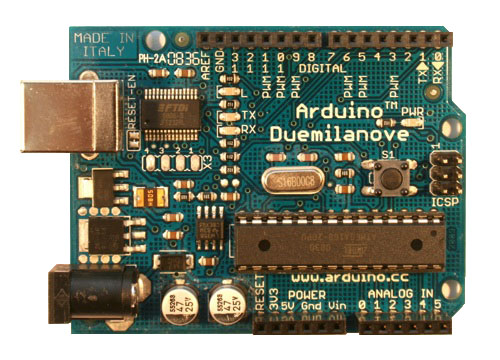
\includegraphics[scale=0.5]{images/ArduinoDuemilanove}

  \caption{Picture of a Arduino Duemilanove. Picture is taken from the Arduino
    homepage: \url{http://arduino.cc/en/Main/ArduinoBoardDuemilanove}.}
  
\end{nonfloatingfigure}

There are different kinds of Arduino boards. All are based on
different ATmega processors from Atmel. The older boards used serial
communication while the newer ones are connected to the computer
through a USB cable, but still using the same serial communication
protocol (i.e., serial through USB). The USB cable also serves as a
power supply.



We will describe the Arduino Duemilanove board we have used, in the
sections that follow, but most information will apply to
the other Arduino boards as well.

\section{Pins}
The Arduino board can connect to several external components through
diverse input and output pins. The pins are split in three physical sections on
the board \textit{power}, \textit{analog in} and
\textit{digital}. Before any IO can happen on a pin, it's mode must be
set. The mode of a pin defines if it is used to read input or
write output. The mode is set by the function \texttt{void pinMode(int
  pinnumber, int mode)} where \textit{pinnumber} is a number between
0-5 for analog and 0-13 for digital and \textit{mode} is either of the constants
\texttt{OUTPUT} or \texttt{INPUT}.

\subsection{Power pins}
% http://arduino.cc/en/Reference/Board?from=Guide.Board
\begin{itemize}
\item Reset: Resets the board when connected to ground.
\item 3V3: Constant 3,3v output
\item 5v: Constant 5v output
\item Gnd: Two ground pins
\item Vin: The voltage supplied by the external power supply.
\end{itemize}

\subsection{Digital pins}

There are 14 digital input and output pins. Six of them can also be
used to generate analog output by PWM (Pulse Width Modulation). It's
possible to read a boolean value \texttt{HIGH} and \texttt{LOW} by the
following function \texttt{bool digitalRead(int pinnumber)} where
pinnumber is a number between 0 and 13. It's possible to write a
boolean value by the following function \texttt{void digitalWrite(int
  pinnumber, int value)} where pinnumber is a number between 0 and 13
and value is either \texttt{HIGH} or \texttt{LOW}.

\subsection{Analog input}
There are 6 analog input pins. It's possible to read a voltage level
from each of them using the function \texttt{int analogRead(int
  pinnumber)} where \textit{pinnumber} is a number between 0 and 5
indicating which pin to read from. The result is given as an integer
in the range from 0 to 1023. It's possible to write a voltage level
(PWM wave, explained below) by the following function \texttt{void
  analogWrite(int pinnumber, int value)} where \textit{pinnumber} is
one of (3,5,6,9,10,11) which is located among the 14 digital pins and
\textit{value} is an integer in the range from 0 to 255. The reason
why the 6 analog output pins is located among the digital IO pins is
that the platform uses PWM to generate the desired voltage level.

\subsubsection{PWM}
\label{sec:pwm}
A description of PWM from the Arduino website follows:
\footnote{\url{http://www.arduino.cc/en/Tutorial/PWM} downloaded the
  28. of April at 17:14}

\begin{quotation}
  Pulse Width Modulation, or PWM, is a technique for getting analog
  results with digital means. Digital control is used to create a
  square wave, a signal switched between on and off. This on-off
  pattern can simulate voltages in between full on (5 Volts) and off
  (0 Volts) by changing the portion of the time the signal spends on
  versus the time that the signal spends off. The duration of "on
  time" is called the pulse width. To get varying analog values, you
  change, or modulate, that pulse width. If you repeat this on-off
  pattern fast enough with an LED for example, the result is as if the
  signal is a steady voltage between 0 and 5v controlling the
  brightness of the LED.

  In the graphic below, the green lines represent a regular time
  period. This duration or period is the inverse of the PWM
  frequency. In other words, with Arduino's PWM frequency at about
  500Hz, the green lines would measure 2 milliseconds each. A call to
  \texttt{analogWrite()} is on a scale of 0 - 255, such that
  \texttt{analogWrite(255)} requests a 100\% duty cycle (always on),
  and \texttt{analogWrite(127)} is a 50\% duty cycle (on half the
  time) for example.

  \begin{nonfloatingfigure}
    \centering
    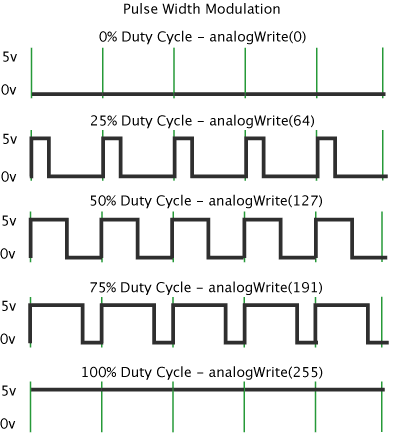
\includegraphics[scale=0.6]{images/pwm}

    \caption{How 0\%, 25\%, 50\%, 75\% and 100\% PWM is measured by an
      oscilloscope. Each vertical line indicates the duty length which Arduino 
      sets approximately to 490Hz.}
    \label{fig:pwm}
  \end{nonfloatingfigure}

  Once you get this example running, grab your Arduino and shake it
  back and forth. What you are doing here is essentially mapping time
  across the space. To our eyes, the movement blurs each LED blink
  into a line. As the LED fades in and out, those little lines will
  grow and shrink in length. Now you are seeing the pulse width.
\end{quotation}



\section{Timer Interrupts}
\label{sec:timer-interrupts}

The ATmega168/ATmega328 processors has three different hardware
timers. One of them (timer 0) is used by Arduino software to provide a
\texttt{millis()} function that gives us the amount of milliseconds
since the timer started and a \texttt{delay} function that actively
holds the processor occupied for a given time period. Timer 0 and 2
uses 8 bit registers and timer 1 uses a 16 bit register. This
effectively means that timer 0 and 2 can't count to more than 255
whereas timer 1 can count to 65535. The registers is incremented at
the speed of the processor, in this case 16MHz, divided by a prescale
factor which can be either of 1 (no scaleing), 8, 64, 256, 1024 for
timer 0 and 1 and either of 1, 8, 32, 64, 128, 256, 1024 for timer
2. The reason why timer 0 and 1 has 2 less prescale factors is that
they can be wired up with an external clock source and setup to
trigger on a falling or rising edge. With a prescale of 256 the
counter is incremented at a rate of $\frac{16000000\mathrm{Hz}}{256} =
62500\mathrm{Hz}$, which makes the counter overflow at a rate of
$\frac{16000000\mathrm{Hz}}{255*256} = \frac{62500\mathrm{Hz}}{255} =
245.1\mathrm{Hz}$ (pr second). This applies to all three timers where the only
2 variables are the prescale and the size of the counter register.

The three timers modes of operation is \texttt{Normal},
\texttt{CTC}(Clear Timer on Compare match), \texttt{Fast PWM},
\texttt{Phase Correct PWM} where \texttt{Normal} and \texttt{CTC} are
the ones of interrest:

\begin{description}
\item[\texttt{Normal}] mode counts from a optionally specified counter
  value (initially default set to 0) and increments until it reaches
  the maximum value 255 where it overruns, restarts from 0, the
  interrupt is triggered and incrementation of the counter
  restarts.

\item[\texttt{CTC}] mode has a predefined top value and optionally
v  specified counter value (initially default set to 0). When the
  counter reaches the defined top value it is cleared to 0, the
  interrupt is triggered and incrementation of the counter
  restarts. This gives better resolution of the counter and thus more
  flexibility than the \texttt{Normal} mode.
\end{description}

The modes of operation is described in detail in \cite[Section 12.7]{atmel8p}.

\subsection{PWM generation}

PWM is generated from these three timers. Pin 5 and 6 are connected to timer 0,
9 and 10 to timer 1 and pin 3 and 11 to timer 2. This means that the frequency
of the PWM signal is controlled by the speed of these counters which again is
determined by the prescale. When an \texttt{analogWrite(pinnumber, value)} is
executed, the associated timer is basically configured to output a \texttt{HIGH}
value as long as the counter is less than the defined \textit{value} and then
\texttt{LOW} until it overflows and restarts. Figurely speaking, to generate a
square wave with a duty cycle of 50\% it must output \texttt{HIGH} on counts $0
\ldots 127$ and \texttt{LOW} on counts $128 \ldots 255$. The actual timer values
is variable with respect to the duty cycle and duty length (Arduino defines the
duty length for \texttt{analogWrite} to approximately 490Hz). This also means
that a particular timer can't be used for anything else if PWM is used.

\section{External Interrupts}
\label{sec:external-interrupts}

Essentially all the pins on the Arduino board supports external
interrupts, though only digital pins 2 and 3 is supported directly by
the Arduino code via the function \texttt{void attachInterrupt(int
  interruptpin, void (* userfunc)(void), int mode)} where
\textit{interruptpin} is either 0 or 1, \textit{userfunc} is the user
function to call when the interrupt triggers and \textit{mode} is one
of \texttt{LOW}, \texttt{CHANGE}, \texttt{RISING} or
\texttt{FALLING}. The \textit{mode} property is special for these two
external interrupt pins, as the other pins only support the
\texttt{CHANGE} mode. The full descriptions of the modes is in the
datasheet of the processor section 10.2.1 ``EICRA - External Interrupt
Control Register A''. To set up external interrupts on the other pins
the user \textit{ckiick} has added an usable header file to the Arduino
playground\footnote{\url{http://www.arduino.cc/playground/Main/PcInt}
  taken 28th of April 2009 at 16:45} also containing an
example of how it works. This header file defines a function
\texttt{void PCattachInterrupt(int interruptpin, void (*
  userfunc)(void), int mode)} where the only difference is that the
\textit{mode} property only supports \texttt{CHANGE}.



\section{Arduino BT}

The Arduino BT board is different from all the other Arduino boards since it
comes with a Bluegiga WT11 Bluetooth chip (from now refered to as WT11 chip)
instead of the USB mount. This means that the board can be programmed and
communicated with through a wireless connection. The communication protocol is
still RS232 so besides the wireless communication nothing is different about
this.

Other main differences as listed at the Arduino
homepage\footnote{\url{http://arduino.cc/en/Main/ArduinoBoardBluetooth} taken
  16th of May at 23:57}:

\begin{itemize}
\item The use of a DC-DC convertor, allowing the board to be powered with a
  minimum of 1.2 V, but with a maximum of 5.5 V. \textbf{Higher voltages or
    reversed polarity in the power supply will kill the board.}

\item A surface-mounted ATmega168 (as with the Arduino Mini). This doubles the
  amount of space available for your sketches and adds three more PWM pins and
  two more analog inputs.

\item Pin 7 is connected to the reset pin of the bluetooth module. 

\item Only use serial communication at 115200 baud; this is the speed that the
  module has been configured to use.
\end{itemize}

As stated digital pin 7 is reserved and connected to the WT11 chip's reset
pin. This means that if a program does a \texttt{digitalWrite(7, HIGH)} and
shortly after does a \texttt{digitalWrite(7, LOW)} the WT11 chip will be
reset. This will however not restore the factory settings of the WT11 chip as
all changes to settings are persistent.

In the below sections it is assumed that the user is using a Unix-like operating
system with Bluetooth associated packages installed, unless otherwise noted.

\subsection{Powering through a USB  cable}

As the board doesn't have the USB mount it is not able to draw power from the
host as most of the other Arduino boards has. This means that the board must be
powered by an external power supply (e.g., batteries). Powering the board when
next to a computer can however still be done through a modified USB cable. As a
standard USB cable consists of 4 wires

\begin{table}[h!]
  \centering
  \begin{tabular}{|c|c|c|}
    \hline
    Contact number & Signal name & Wire colour \\ \hline
    1 & VCC & Red \\ \hline
    2 & D- & White \\ \hline
    3 & D+ & Green \\ \hline
    3 & GND & Black \\ \hline
  \end{tabular}
  \caption{USB Connector Termination Data. Described in the USB 2.0
    specification \cite[Table 6-1 ``USB Connector Termination Assignment'']{usb20} }
  \label{tab:ArduinoBT:Connector_Termination_Data}
\end{table}

According to the USB 2.0 specification \cite[Table 7-7 ``DC Electrical
Characteristics'']{usb20} the VCC wire supplies a minimum of 4.75v and a maximum of
5.25v which is no problem as the Arduino BT board can handle up to 5.5v and as
low as 1.2v. There is however always a slight possibility of faulty equipment
which could damage the board.

The wire colours for a standard USB 2.0 cable are defined in the
specification \cite[Figure 6-2 ``USB Standard Detachable Cable Assembly'']{usb20}
but it is not all manufactures that comply with this.

To construct the USB power cable all that needs done is to cut off the connector
opposite of the Standard-A connector, which is the one that fits in the
computer. Next strip off the a few cm of the PVC jacket and the copper/aluminium
shield on the cable so the four wires are free. Then cut away the 2 data wires
(green and white) and strip off 0.5cm of the VCC and GND wires insulations (red
and black). Now the two stripped wires can be connected to the Arduino BT board
through the power socket (X1). Remember not to reverse the polarity when
connecting the two wires, ore else the board cold be damaged.

\subsection{Binding with the device}

Before the board can be programmed or communicated with, it must be binded with
a host. To bind with a Bluetooth device, its MAC address is needed. A list of
names and MAC addresses of all Bluetooth devices in the area can be found with
the following command:

\begin{verbatim}
hcitool scan
\end{verbatim}

A factory Arduino BT board is always named \textit{ArduinoBT} and has the PIN
12345. There are at least 2 ways of handling Bluetooth PIN authentication. The
simplest ways is to put the PIN and nothing else in the file
\textit{/etc/bluetooth/pin} before binding with the device this however can be
complicated when binding with multiple devices with different PIN as the file
can only contain a single PIN at a time. The other way is to use
\texttt{bluetooth-applet} (Gnome) or \texttt{kbluetooth4} (KDE), which both
places a icon in the tray and queries the user for a PIN when required by the
Linux Bluetooth stack.

Whichever way is used, the host can now bind with the Arduino BT board with the
following command

\begin{verbatim}
rfcomm bind rfcommX xx:xx:xx:xx:xx:xx 1
\end{verbatim}

where \texttt{rfcommX} is the desired host device that is to be used (e.g.,
\texttt{rfcomm0}), \texttt{xx:xx:xx:xx:xx:xx} is the boards MAC Address and
\texttt{1} is the channel to be used. A factory Arduino BT board has only
enabled \texttt{SSP} (Serial Port Profile) and thus this is located on channel
1. It is possible to query which Bluetooth profiles the Arduino BT board exposes
by the following command

\begin{verbatim}
sdptool browse xx:xx:xx:xx:xx:xx
\end{verbatim}

To find the channel, just locate \texttt{SPP} in the returned list and see what
channel the \texttt{rfcomm} protocol is associated with.

\subsection{Important program setup}

When creating a program for the Arduino BT it is important to remember a few
things in the \texttt{setup()} function. This is to ensure that the WT11 chip is
always configured when the program starts. The WT11 chip remembers its settings
even if it loses power. This means that if the settings are change at some point
of the program execution then at least the basic settings will be set to a known
default when the program is restarted. It is however still possible to change
the settings of the WT11 chip so it won't accept connections from any
hosts. This is addressed in the below sections.

\begin{table}
  \centering
\begin{verbatim}
  pinMode(7, OUTPUT);
  Serial.begin(115200);
  digitalWrite(7, HIGH);
  delay(10);
  digitalWrite(7, LOW);
  delay(2000);

  Serial.println("SET BT PAGEMODE 3 2000 1");
  Serial.println("SET BT NAME ARDUINOBT");
  Serial.println("SET BT ROLE 0 f 7d00");
  Serial.println("SET CONTROL ECHO 0");
  Serial.println("SET BT AUTH * 12345");
  Serial.println("SET CONTROL ESCAPE - 00 1");
  Serial.println("SET CONTROL BAUD 115200,8n1");
\end{verbatim}
  \caption{asd}
  \label{tab:ArduinoBT:Initial_Setup_code}
\end{table}


The WT11 chip is connected to the ATmega processor by its RX and TX lines, which
means that communication is done through Arduino's serial communication
capabilities. The WT11 chip communicates at a baud rate of 115200 thus it is
important to use this speed in the \texttt{Serial.begin} function. Even though
the WT11 chip's iWRAP firmware can be changed to use another baud rate, this is
not recommended and will most likely not work. The name that should be visible
when searching to Bluetooth devices is configured by the \textit{SET BT NAME}
command, and the PIN is configured by\texttt{SET BT AUTH *} command. Other iWRAP
commands and their definitions can be seen in the ``iWRAP User Guide''.

\subsection{Communication without Bluetooth}

If the WT11 chip is configured in a way such that it refuses connections or in
some other way that the ATmega processor cannot be programmed, you need to reset to
factory settings (by doing a firmware update) or by changing the individual
settings back to something that works. 

Before settings on the WT11 chip can be changed, they must be directly sent to
it. This can be done by using a 3.3v USB to RS-232 serial converter\footnote{E.g., a
  breakout board with FTDI's FT232RL chip, which is widely available and can be
  used to update the firmware using the DFU protocol as well.
  \url{http://www.sparkfun.com/commerce/product_info.php?products_id=718}} and
connect it to the WT11 chips \texttt{RX} and \texttt{TX} pins which can be
located at the two solder points \texttt{JP1} directly underneth the WT11 chip
on the bottom side of the Arduino board. As \texttt{RX} is the receive line and
\texttt{TX} is the transmit, it is important to cross these two\footnote{Serial
  converter RX goes to WT11 TX and serial converter TX goes to WT11 RX} when
connecting the serial converter and the WT11 chip. No damage will happen if the
lines aren't crossed, but no communication will be able to take place.

There can be some timing issues if using an external power source while using
the serial convert, so it is highly recommended to use the serial converters
3.3v power supply feature.

The most common issues and solutions is
 
\begin{itemize}
\item If control echo has been enabled it will not be possible to program the
  ATmega processor as the bootloader will receive messages from the WT11 chip at
  bootup and thus fail when waiting for control characters. The solution to this
  is to disable control echo by sending the command \texttt{SET CONTROL ECHO 0}.

\item If the SPP (Serial Port Profile) has been disabled, no host can make a
  serial (rfcomm) connection and thus not make any serial communication (program
  the ATmega processor). The solution to this is to enable the SSP again by sending
  the following command \texttt{SET PROFILE SPP on} and then reset the WT11 chip
  by putting high on pin 7 for a short while or sending the command
  \texttt{RESET}.

\item If bluetooth connection is restored, the serial converter is still
  connected and any attempt to program the ATmega processor fail. Solution to this is
  that the serial converter must not be connected to the Arduino board while
  trying to program the ATmega processor. 

  In fact the serial converter interferes with the signals whether it is
  connected to the WT11 chip or ATmega processor (digital pins 0 and 1). This results
  in communication only goes between the serial converter and the chip it is
  connected to. So whenever communication between the ATmega processor and the WT11
  chip is desired, the serial converter must be disconnected.
\end{itemize}

\subsection{iWRAP interface}

By default the WT11 chip uses the iWRAP firmware which enables the user to
access Bluetooth functionality with simple ASCII commands sent by a serial
interface. The Arduino BT board is shipped with the iWRAP firmware version 2.2.0
as default. If the Arduino BT board is used with a host that takes care of the
binding then there is properly no need for changing any of the WT11 chips
settings. But if the Arduino BT board is the one who needs to do the binding
with another Bluetooth device then it is necessary to change the settings and
therefor also shift into command mode. A thorough description of the different
iWRAP settings and commands can be seen in the iWRAP 2.2.0 User
Guide \cite{iWRAP220UG}.


\subsubsection{iWRAP modes}

iWRAP can be in three different modes: command,data and mux mode (multiplexing
mode).

Command and data mode are the default behaviour. Before sending any commands to
the iWRAP interface it must be in command mode. The iWRAP interface is always in
command mode when there is no active connections. When a connection is made
iWRAP automatically switches to data mode on this connection.  The mode can be
switched back to command mode by waiting at least one second, sending the
sequence \texttt{esc esc esc} and wait at least one second (\texttt{esc} is the
defined escape character\footnote{The escape character is defined by the iWRAP
  command \texttt{SET CONTROL ESCAPE}}). When in command mode the \texttt{LIST}
command will list all active connections and \texttt{SELECT} \textit{link\_id}
command will switch to data mode on the specified connection. Command/data mode
has the advantage of being easy and fairly intuitive when operating one a small
amount of active connections (preferably only one connection) but when multiple
connections is used the mode switching becomes quite a bottleneck as iWRAP needs
to be in data mode on the desired connection to receiving data and if it is in
command mode or data mode on another connection the data is stored in a buffer
and thus could potentially be lost if the buffer overflows before the connection
is selected.

This can however be solved by using multiplexing mode. In multiplexing mode data
and command mode is melted into one mode and it uses a special protocol which
doesn't accept normal iWRAP ASCII commands. Instead the multiplexing protocol is
a ASCII list of space separated hex values that contains some control segments
which defines whether the data part is a control (iWRAP command) sequence or
which connection the data sequence should be sent to or is received
from. \Fref{tab:multiplexing_protocol} illustrates the multiplexing frame
format.

\begin{table}[h!]
  \centering
  \textsf{
    \begin{tabular}{|l|l|l|l|}
      \hline
      \textbf{Length:} & \textbf{Name:} & \textbf{Description:} & \textbf{Value:} \\ \hline
      8 bits & SOF & Start of Frame & \texttt{0xBF} \\ \hline
      8 bits & LINK & Link ID & \texttt{0x00}--\texttt{0x08} or \texttt{0xFF} for
      control commands \\ \hline
      6 bits & FLAGS & Frame Flags & \texttt{0x00} \\ \hline
      10 bits & LENGTH & Size of data field in bytes & - \\ \hline
      0-800 bits & DATA & Data & - \\ \hline 
      8 bits & nLINK & LINK \texttt{xor} \texttt{0xFF} & - \\ \hline 
    \end{tabular}
  }
  \caption{Multiplexing frame format as described in Table 4 of the iWRAP 2.2.0 User
    Guide}
  \label{tab:multiplexing_protocol}

\end{table}

When multiplexing mode is enabled\footnote{To enable multiplexing mode send the
  iWRAP command \texttt{SET CONTROL MUX 1}}, it can be disable by the following
sequence \texttt{BF FF 00 11 53 45 54 20 43 4f 4e 54 52 4f 4c 20 4d 55 58 20 30
  00} which should be send as its ASCII representation without spaces. A python
script that demonstrates this can be seen in \Fref{sec:python-demux-script}.

The sequence breaks down to the following

\begin{center}
  \begin{tabular}{|l|p{300pt}|}
    \hline 
    \textbf{Name:} & \textbf{Description:} \\ \hline
    \textsf{SOF} & Is always \texttt{0xBF} \\ \hline
    \textsf{LINK} & Is \texttt{0xFF} as it is a control command \\ \hline
    \textsf{FLAGS} & Is always \texttt{0x00} \\ \hline
    \textsf{LENGTH} & Is \texttt{11} (length of data is 17 characters) \\ \hline
    \textsf{DATA} & Is \texttt{53 45 54 20 43 4F 4E 54 52 4F 4C 20 4D 55 58 20
      30} which is the hex representation of \texttt{SET CONTROL MUX 0} \\ \hline
    \textsf{nLINK} & is \texttt{0x00} as \texttt{0xFF xor 0xFF = 0x00} \\ \hline
  \end{tabular}
\end{center}
 
iWRAP commands should not end with ``$\backslash$r'' or
``$\backslash$r$\backslash$n'' when used in a multiplexing frame.

The iWRAP 2.2.0 User Guide states that there can be used four simultaneous
connections in multiplexing mode, though iWRAP 3.0.0 User Guide \cite[section
6.20.3, page 120]{iWRAP300UG} states that

\begin{quote}
  In MUX mode the processor of the module is highly utilised and on the edge of
  its performance. This may be seen as a instability of Bluetooth connections,
  especially if 3 or more connections are used or data rate is high.
\end{quote}

\noindent
and suggests to use \texttt{SNIFF} mode and optimise the bluetooth packet size
by using the MTU option in the \texttt{CALL} command to leave more time for the
processor to parse the multiplexing protocol. 

Section 3 of the iWRAP 2.2.0/3.0.0 User Guide covers the three iWRAP modes in
depth.


\subsubsection{Firmware update}

Bluegiga Technologies support 2 ways of updating the firmware. A proprietary SPI
protocol that uses a SPI interface or a open DFU (Device Firmware Update)
protocol\footnote{The DFU protocol description can be retrieved by contacting
  the Bluegiga support team.} which uses a DFU interface over a UART or USB connection.

The downside of the SPI interface is that 

\begin{itemize}
\item it requires a special SPI cable which basically is a parallel to SPI
  converter.

\item The proprietary BlueSuite software supplied by Bluegiga Technologies used
  to update the firmware is only released for Windows\footnote{It has not been
    confirmed whether or not it works on Linux through Wine}.

\item It is necessary to have direct access to the WT11 chip's SPI interface.
\end{itemize}

Downside of DFU interface is that 

\begin{itemize}
\item it requires special version of the firmware which can be obtained by
  contacting the Bluegiga support team.

\item It is however not all firmware versions that can be update through the DFU
  interface\footnote{``... For example iWRAP 2.1.0 can not be updated to iWRAP
    2.2.0, since the DFU boot loader code has changed''
    (\url{http://techforum.bluegiga.com/faq_item?id=10377296} 17th of may at
    19:36)}.

\item It is necessary to have access to the WT11 UART or USB
  interface. This can however be done by uploading a program to the host
  processor through Bluetooth and make it do the firmware upgrade.
\end{itemize}

Bluegiga Technologies recommends to buy or build a OIK (OnBoard Installation
Kit) \cite{oik_chematic}, but the Arduino community has posted an alternative
schematic \cite{oik_chematic_arduino} which we couldn't get to work.

Instead the DFU protocol was used to successfully update the firmware on one of
the Arduino BT boards by connecting a breakout board to the RX and TX pins of
the WT11 chip. The DFU Wizzard application (used to upload the firmware) however
didn't work properly when trying to download a backup of the WT11 chips current
firmware which is a prerequisite for uploading new firmware. This can however be
circumvented by pointing the backup location in the DFU Wizzard application to a
copy of a arbitrary firmware DFU file. This makes the application think that a
backup has already been made and thus upload of new firmware is allowed.

\chapter{Discovered Flask issues}
We've detected a few problems with the current Flask implementation,
that we think should needs to be resolved. The same problems appears
in Fladuino, as we haven't set much time aside to look for solutions
to the problems.

\begin{itemize}
\item Pattern-matching isn't handled correctly. The following program
  is compiled as if the two first cases where overlapping (i.e., the
  second case would be ignored)
\begin{verbatim}
f (1, (1, x)) = 2
f (1, (2, x)) = 3
f (2, _) = 3
\end{verbatim}

\item In Haskell, 42 can both be interpreted as an $Integer$, a
  $Double$, or any other member of the $Num$-type class. In Red this
  isn't the case and thus \texttt{negate} and \texttt{(-)}, which
  are defined by \verb|negate x = 0 - x|, only works for
  integers.(Related to the lack of type-classes). Instead, you can
  define a negation function for \textit{Doubles}, by: \verb|neg x = 0.0 - x|.

\item This is more of an improvement point on Flask, than a issue. We
  think the Flask programmer should have a way of adding a dataflow
  subgraph to the initialisation phase of the generated program.
\end{itemize}

\chapter{Code examples}

\section{Python demux script}
\label{sec:python-demux-script}

This is a python script that sends the iWRAP command \texttt{SET CONTROL MUX 0}
to disable multiplexing mode. This assumes that the breakout board is connected
to the WT11 chips serial communication pins and connected to the computer at
\textit{/dev/ttyUSB0}.

\begin{verbatim}
#!/usr/bin/python

# sets str to '\xbf\xff\x00\x11SET CONTROL MUX 0\x00'
str = 'BFFF001153455420434f4e54524f4c204d5558203000'.decode("hex")

f = open('/dev/ttyUSB0', 'w')
f.write(str)
f.close()
\end{verbatim}

\section{valueOf function}
\label{sec:valueOf}

\begin{verbatim}
valueOf :: forall a d. (Reify a, AnalogInputDevice d) => d -> S a -> S Integer
valueOf d a = S $ do
    sa   <- unS a
    addStream "valueOf"
              tau_b
              (DeviceRead sa $ uniqueId d)
              genHs
              genC $ \this -> do
    addDevice d
    connect sa this tau (varIn this "")
  where
    tau :: H.Type
    tau = reify (undefined :: a)
    tau_b :: H.Type
    tau_b = reify (undefined :: Integer)

    genHs :: SCode m -> FladuinoM ()
    genHs this =
        addCImport c_v_in [$ty|$ty:tau -> ()|] [$cexp|$id:c_v_in|]
        where
          v_in    = varIn this ""
          c_v_in = show v_in

    genC :: SCode m -> FladuinoM ()
    genC this = do
        tauf <- toF tau
        tauf_out <- toF tau_b
        (params, ce_params) <- ToC.flattenParams tauf
        ce_out <-  hcall v_out $ ToC.CLowered tauf_out [$cexp|v|]
        let stms = genReadCode d "v"
        addCFundef $ [$cedecl|
void $id:c_v_in($params:params)
{
  unsigned int v;
  $stms:stms;
  $exp:ce_out;
}
|]
        where
          v_in   = varIn this ""
          c_v_in = show v_in
          v_out = s_vout this
\end{verbatim}

\end{document}
